\section{Multivariate analysis}
\label{sec:mva}

At the end of the loose cut-based analysis,
by combining the three event topologies,
we obtain a signal significance of $S/\sqrt{B}\simeq 0.8~(1.4)$
with all backgrounds (only QCD $4b$) considered.
%
This section describes how this signal significance
 can be enhanced when the cut-based analysis
 is complemented by multivariate techniques.
%
 These are by now a mature tool
 in high-energy physics data analysis, opening
 new avenues to improve the performance
of many measurements and searches at high-energy colliders.
%
In particular, the classification of events into
signal and
background processes by means of MVAs is
commonly used in LHC
applications~\cite{Baldi:2014pta,Aaltonen:2012qt,
  Wardrope:2014kya,Chatrchyan:2013zna,Dall'Osso:2015aia,Kang:2015uoc}.

In this section, first we present the specific MVA that we use,
based on feed-forward multi-layer neural networks.
%
Then we introduce the input variables that are
used in the MVA, including the jet substructure
variables, and then present the signal significance obtained
by applying the MVA.
%
Then we assess the robustness of the MVA strategy in
the case of significant contamination from pileup.

\subsection{Deep artificial neural networks}

The specific type of  MVA that we use to
disentangle signal and background events is
a multi-layer feed-forward artificial neural network (ANN),
known as a {\it perceptron}.\footnote{This type of ANNs are the same
  as those used to parametrize Parton Distribution Functions
in the NNPDF global analyses~\cite{DelDebbio:2004qj,Ball:2008by,Ball:2011mu,Ball:2010de}.}
%
This family of ANNs are also known as {\it deep neural networks},
due to their multi-layered architecture.
%
The MVA inputs are a set of kinematic variables describing the
signal and background
events which satisfy the requirements of the
cut-based analysis.
%
The output of the trained ANNs also allows for the identification,
in a fully automated way,
of the most relevant variables in the discrimination between 
signal and background.

In this work, the ANN that we use has the following architecture.
\be
\label{eq:nn1}
N_{\mathrm{var}}\times5\times3\times1 \, ,
\ee
where $N_{\mathrm{var}}$ represents the number of input variables for the MVA,
which is different in the resolved, intermediate, and boosted categories.
%
All neural-network layers use a sigmoid activation function, allowing
for a probabilistic
interpretation of the ANN output.
%
In Fig.~\ref{fig:nnarch} we show an illustrative
example of an ANN used in this work, corresponding 
to the case of the boosted category (thus $N_{\mathrm{var}}=21$, as we explain below).

%%%%%%%%%%%%%%%%%%%%%%%%
\begin{figure}[t]
  \begin{center}
      \vspace{-1cm}
  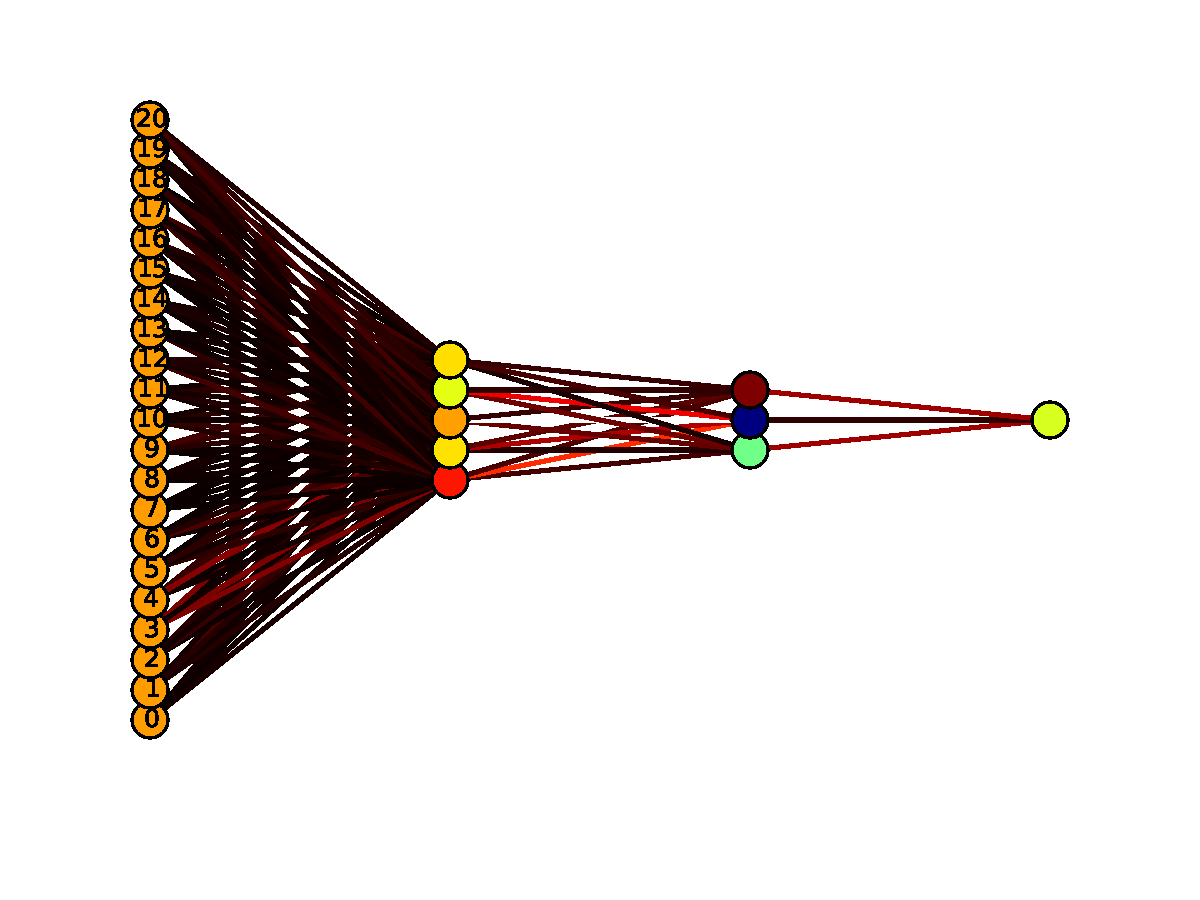
\includegraphics[width=0.90\textwidth]{plots/bst_nnarch_noPU.pdf}
  \vspace{-2cm}
  \caption{\small Schematic of the Artificial
    Neural Network (ANN)
    used for the analysis of the
    boosted
    category, with $N_{\rm var}=21$ input variables and thus
    the same number of neurons
  in the first layer.
  %
  The color code in the neuron connections (the weights) is a heat map obtained
  at the end of the Genetic Algorithms training,
  with red indicating larger values and black indicating smaller values.
}
\label{fig:nnarch}
\end{center}
\end{figure}
%%%%%%%%%%%%%%%%%%%%%%%

The training of the ANN for the signal/background classification task
proceeds as follows.
%
Given a set of $N_{\mathrm{var}}$  kinematic variables $\{k\}_i$ associated with the event $i$, and a set of neural network weight
parameters $\{\omega\}$, we interpret the neural network output $y_i$
(the activation state of the
neuron in the last layer)
as the probability that the event $i$ originates from the signal process,
\be
y_i = P(y^\prime_i=1|\{k\}_i, \{\omega\} )\, ,
\ee
where $y_i^\prime$ represents the true classification of the event $i$, {\it i.e},
$y^\prime_i = 1$ for signal and $y^\prime_i = 0$ for background events.
%
With this interpretation, our general classification probability including background events is given by
\be
P(y_i^\prime|\{k\}_i, \{\omega\}) = y_i^{y^\prime_i}(1-y_i)^{1-y^\prime_i} \, ,
\ee
consequently we can define an error function $E(\{\omega\})$
to be minimized during the ANN training. In this case, the error function is
the cross-entropy function, defined as
 \bea
 &&E(\{\omega\}) \equiv -\log\left(\prod_i^{N_{\text{ev}}} P(y_i^\prime|\{k\}_i, \{\omega\})\right)\nonumber\\
 &&=
 \sum_i^{N_{\text{ev}}} \lc y^\prime_i\log{y_i} + (1-y^\prime_i)\log{(1-y_i)}\rc \, ,
 \label{cross-entropy}
 \eea
 where $N_{\text{ev}}$ is the number of
 Monte Carlo events that are used for the ANN training.
 %
 The ANN is trained both on the signal and background MC events,
 so it is important to ensure that the input MC sample is large enough
 to avoid contamination from MC statistical fluctuations.
 
 The training of the neural networks therefore consists of the
 minimization of the cross-entropy error,
 Eq.~(\ref{cross-entropy}), which in this work is achieved using a
 Genetic Algorithm (GA).
 %
 Genetic Algorithms~\cite{quevedo,tau,Abel:2014xta,Nesseris:2012tt} are
 non-deterministic
 minimization strategies suitable for the solution
 of complex optimization problems, for instance when a very large number
 of quasi-equivalent minima are present.
 %
 GAs are inspired on natural selection processes
 that emulate biological evolution. 
 %
 In our case, the GA training is performed for a very large 
 number of generations, $N_{\rm gen}=5\cdot 10^{4}$, to avoid the risk of
 under-training.
 %
 We have verified that if a much larger number of generations
 are used, the results are unchanged.
 %

 In addition,
 in order to avoid the possibility of over-fitting,
 we have used a cross-validation stopping
 criterion, in particular the same one as
 that used in the NNPDF3.0 analysis~\cite{Ball:2014uwa}.
 %
 This cross-validation proceeds by dividing the input MC dataset into two disjoint sets,
 using one for training the ANN and the other for validation: the optimal
 stopping point is then given by the minimum of the error function
 Eq.~(\ref{cross-entropy}) to the validation sub-sample.
 %
 This indicates the point where
the ANN begins to train upon  statistical fluctuations
in the input MC samples, rather than learning
the underlying (smooth) physical  distributions.
 
 \subsection{Input kinematic variables}
 \label{sec:input}

In this work we use different sets of
input variables for the three categories.
%
In the case of large-$R$ jets, we  exploit the available
information  on jet substructure.
%
For the three categories, boosted, intermediate and resolved,
the following common variables are used as input to the MVA:
\begin{itemize}
\item The transverse momenta of the leading and subleading Higgs, $p_{T,h_1}$ and $p_{T,h_2}$.
\item The transverse momentum of the reconstructed Higgs pair, $p_{T,hh}$.
\item The invariant masses of the leading and sub-leading Higgs candidates, $m_{h,1}$ and $m_{h,2}$.
\item The invariant mass of the reconstructed Higgs pair, $m_{hh}$.
\item The separation in the $\phi$--$\eta$ plane
  between the two Higgs candidates, $\Delta R_{hh}$.
  \item The separation in $\eta$  between the two Higgs candidates, $\Delta \eta_{hh}$.
\item The separation in $\phi$  between the two Higgs candidates, $\Delta \phi_{hh}$.
\end{itemize}
In addition, in the boosted category we use
  the transverse momenta of the leading, $p_{T,h_{1,1}}$ and $p_{T,h_{1,2}}$ and
  sub-leading, $p_{T,h_{2,1}}$ and $p_{T,h_{2,2}}$, Higgs candidate AKT03 subjets.
  %
  In the resolved category instead,
  the corresponding variables are
  the transverse momenta $p_{T,i}$ of the four leading 
  $b$-tagged small-$R$ jets in the event.
  %
  In the intermediate category, we use the
  transverse momenta of the subjets
  from the large-$R$ jet $p_{T,h_{1,1}}$ and $p_{T,h_{1,2}}$ and the
 transverse momenta $p_{T,i}$ of the two leading 
  $b$-tagged small-$R$ jets.
  %
 Therefore, we have 13 variables which are common to the three categories.

 In the boosted and intermediate categories, we also include the jet substructure
 variables introduced in Sect.~\ref{sec:analysis} for the
 large-$R$ jets: the $k_t$ splitting scales
 $\sqrt{d_{12}}$, the ratio of 2-to-1 subjettiness $\tau_{12}$,
 and the ratios of energy correlation functions $C^{(\beta)}_2$ and
 $D_2^{(\beta)}$.
 %
 This leads to
 a total of $N_{\mathrm{var}}=13,17$ and 21 variables for the
resolved, intermediate, and boosted categories, respectively.


Given that the MVA is able to identify the most discriminatory variables
in an automated way,
and to suppress those which have little effect, it is advantageous to
include a wide array of input variables.
%
This is one of the main advantages of ANNs in this context: 
their inherent redundancy means that 
adding additional information, even if carries very little weight,
should not degrade
the classification power of the MVA.

\subsection{MVA results}
\label{sec:signalsignificance}

We now present the results of the MVA, first without PU, and then
later including the effects of PU.
%
First of all, in Fig.~\ref{fig:nnresponse} we show the distribution of
the ANN output at the end of the GA minimization,
separately for the
boosted, intermediate and resolved categories.
%
All distributions are normalized so that their integral
  adds up to one.
%
The  separation between signal and background is achieved by introducing
a cut, $y_{\rm cut}$, on the ANN output, so that MC events with $y_i\ge
y_{\rm cut}$ are classified as signal events, and those with
 $y_i <
y_{\rm cut}$ as background events.
%
Therefore,
the more differentiated the distribution of the ANN output is
for signal and background events, the more efficient
the MVA discrimination will be.

%%%%%%%%%%%%%%%%%%%%%%%%%%%%
\begin{figure}[t]
\begin{center}
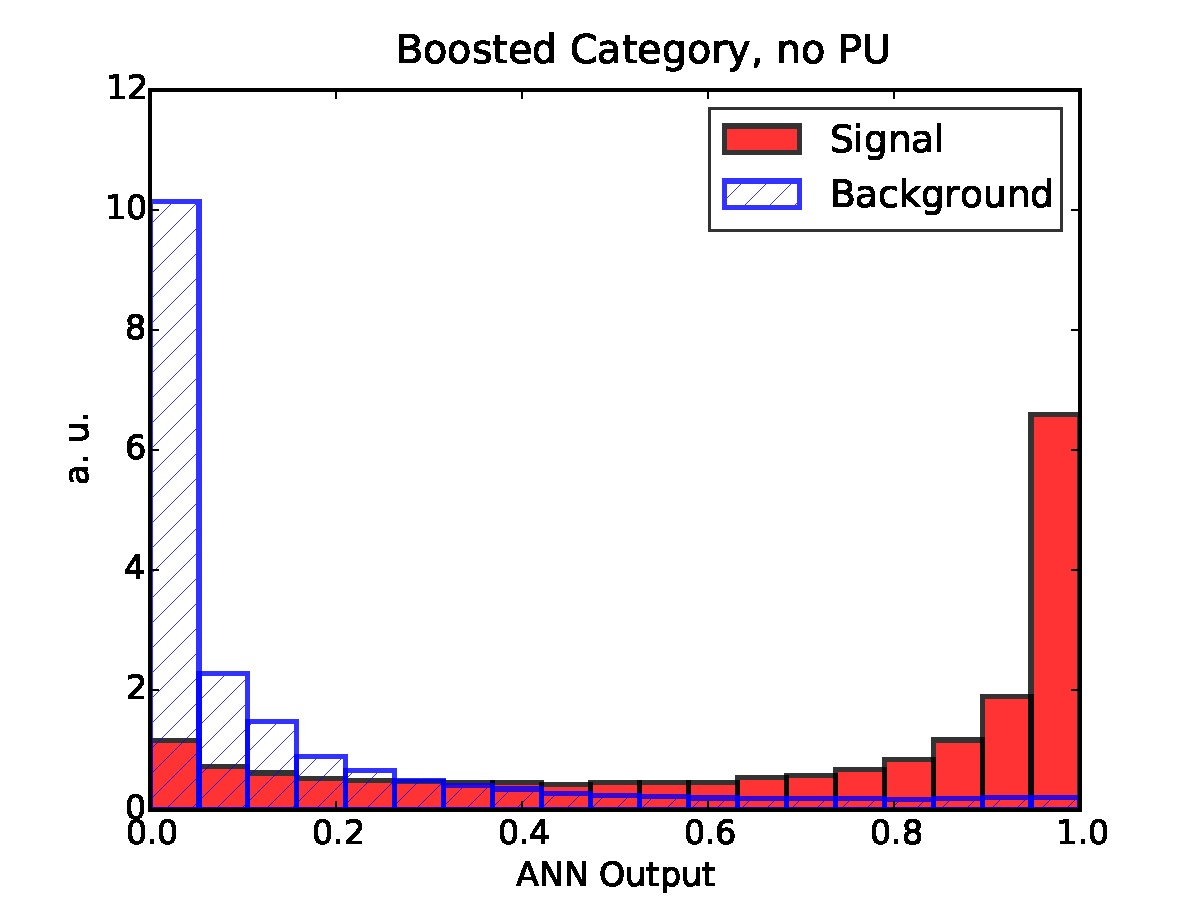
\includegraphics[width=0.65\textwidth]{plots/Boosted_disc_noPU.pdf}
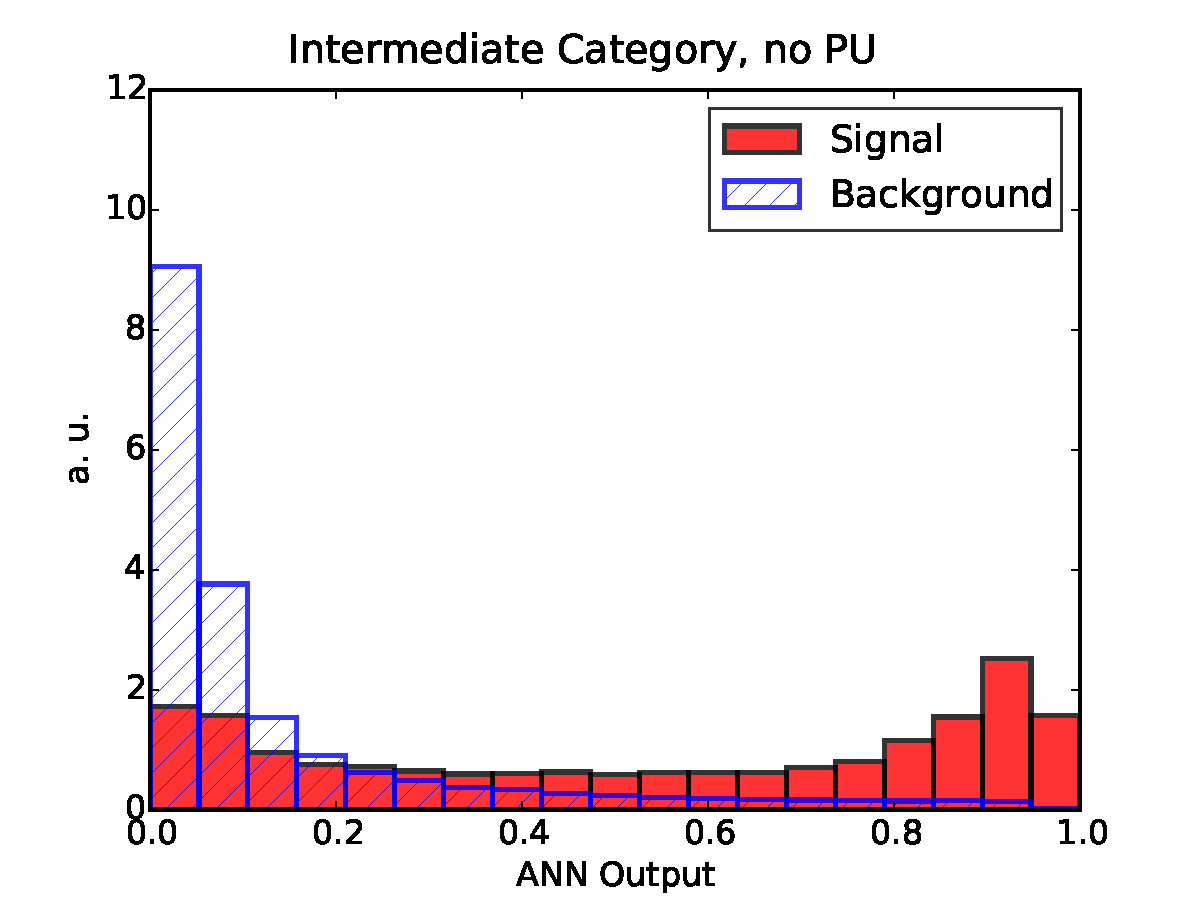
\includegraphics[width=0.48\textwidth]{plots/Intermediate_disc_noPU.pdf}
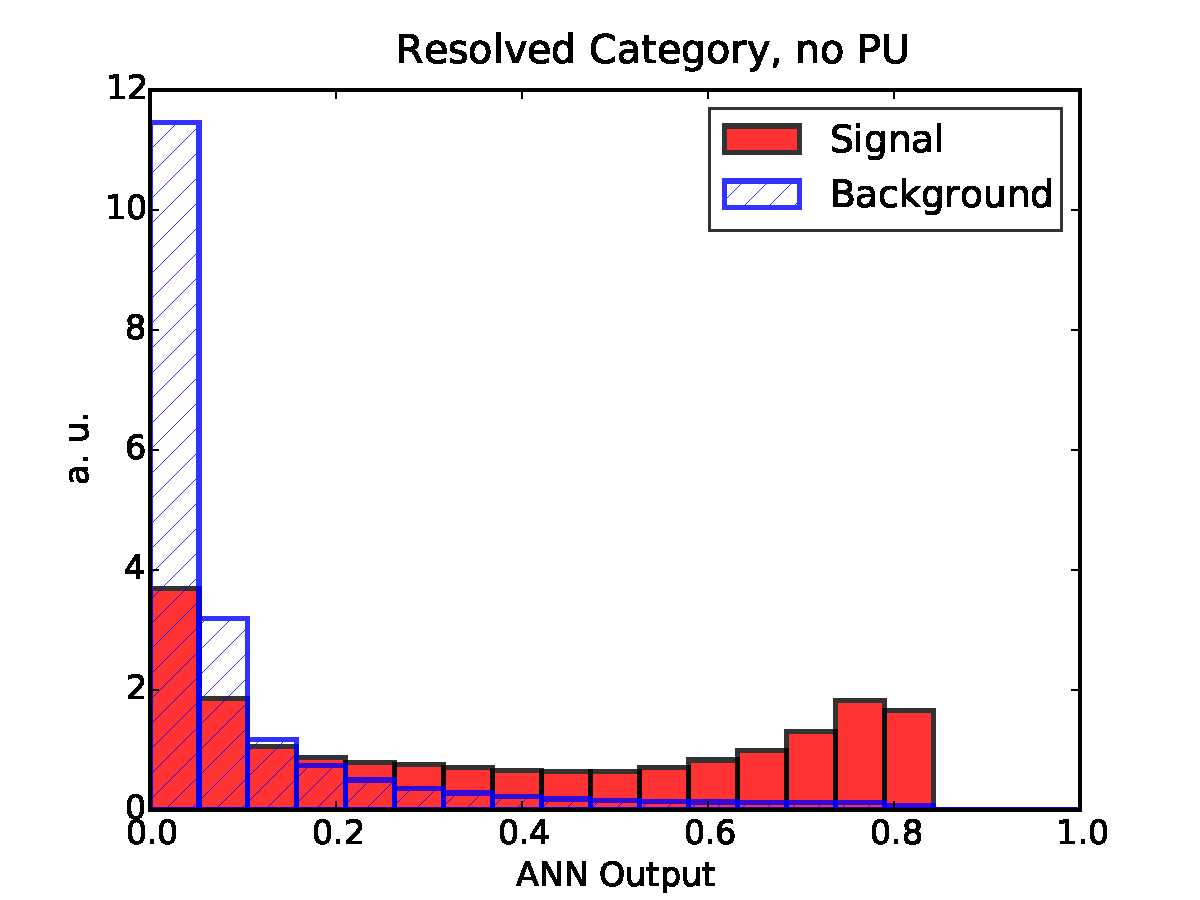
\includegraphics[width=0.48\textwidth]{plots/Resolved_disc_noPU.pdf}
\caption{\small The distributions, at the end of the
  GA training, 
  for the signal and background MC events in the three categories:
  boosted (upper plot), intermediate (lower left plot) and
  resolved (lower right plot), as a function of the ANN output.
}
\label{fig:nnresponse}
\end{center}
\end{figure}
%%%%%%%%%%%%%%%%%%%%%%%

From Fig.~\ref{fig:nnresponse} we see that in the boosted category the MVA can produce
a clear discrimination between signal and background, with the two distributions
forming peaks at their respective optimal limits.
%
This indicates that introducing a suitable cut
$y_{\rm cut}$
in the ANN output will substantially reduce the background,
while keeping a reasonable signal efficiency.
%
The performance of the MVA discrimination is similar,
although slightly worse, in the intermediate
and resolved categories.


The results for the signal selection efficiency and the 
background rejection rate as a function of the cut in the ANN output
$y_{\rm cut}$
define the so-called  Receiver-Operating Characteristic (ROC)
curve, shown in Fig.~\ref{fig:exampleroc}.
%
It is clear that we can achieve  high signal efficiency by using
a small value of $y_{\rm cut}$, but such a choice would be
affected by poor background
rejection.
%
Conversely, using a higher value of the cut will increase background rejection at the
cost of dropping signal efficiency.
%
As could already be inferred from the distribution of neural
networks output in Fig.~\ref{fig:nnresponse}, we find
that our MVA is reasonably efficient
in discriminating signal over background.
%
The performance is best in the case of the boosted category,
and then slightly worse in the resolved
and intermediate categories, consistent with the distributions of
the ANN outputs in
Fig.~\ref{fig:nnresponse}.
%

%%%%%%%%%%%%%%%%%%%%%%%%%%%%%%%%%%%%%%%%%%%%%%
\begin{figure}[t]
\begin{center}
  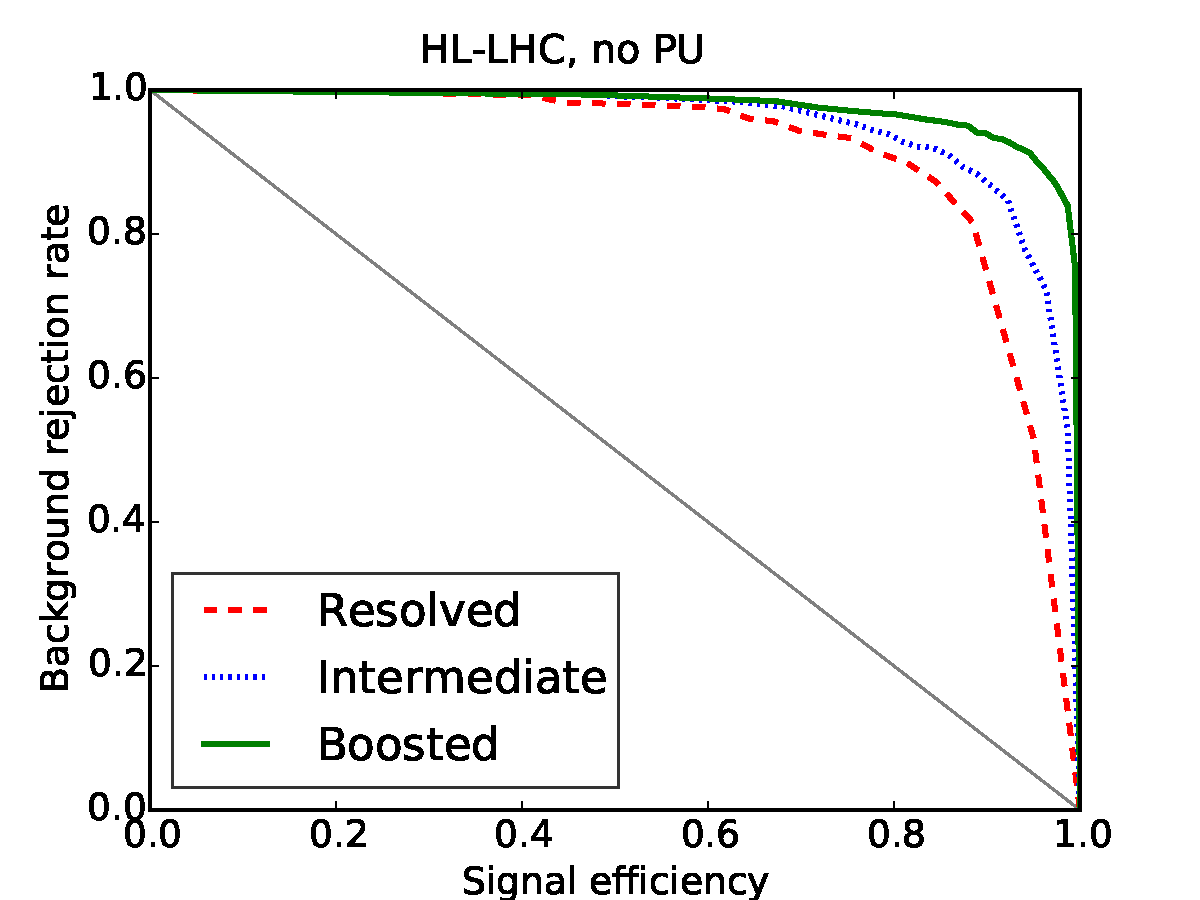
\includegraphics[width=0.49\textwidth]{plots/roc_noPU.pdf}
  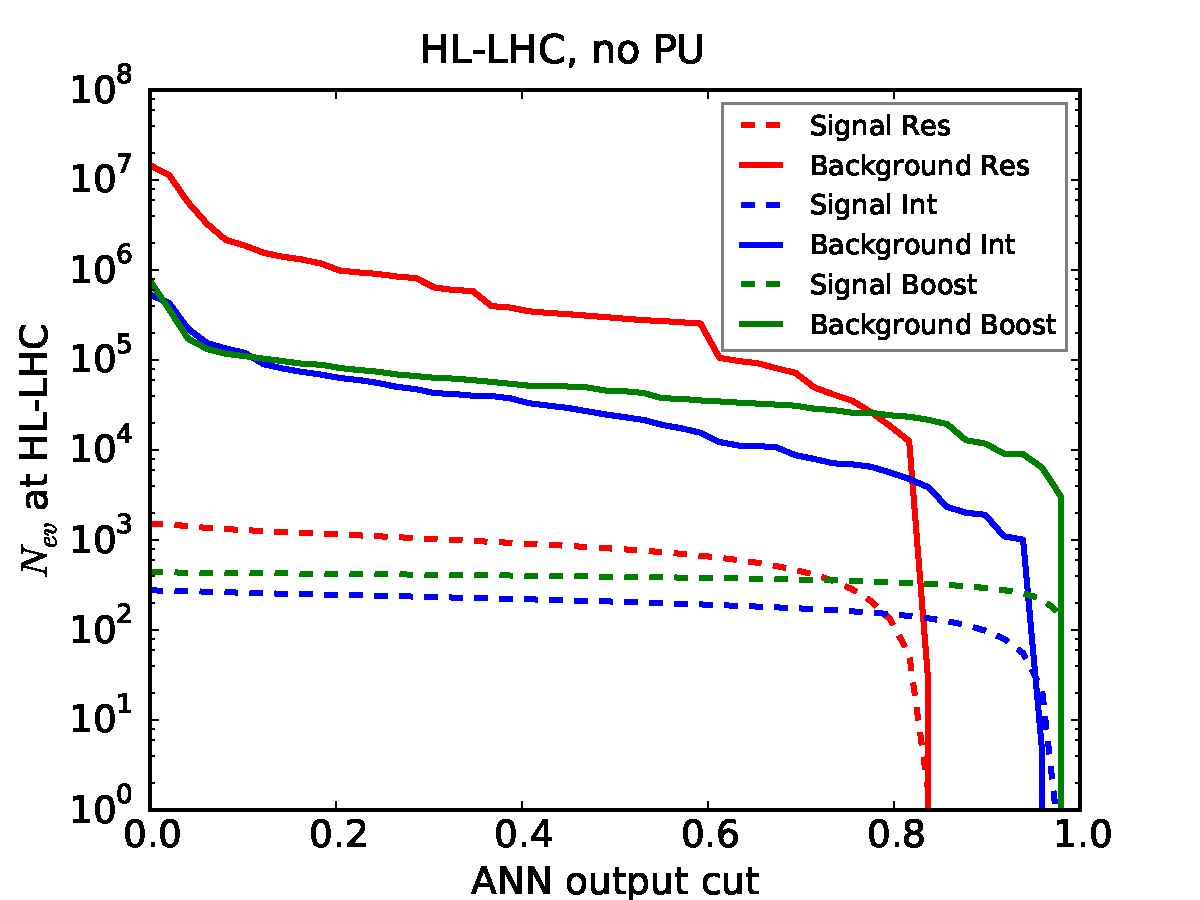
\includegraphics[width=0.49\textwidth]{plots/nev2_noPU.pdf}
\caption{\small Left: ROC curve for the background rejection rate as a function of the signal
  selection efficiency, as the cut $y_{\rm cut}$
  in the ANN output is varied.
  %
  Right: Number of signal (dashed) and background (solid)
  events expected at the HL-LHC as a function of the $y_{\rm cut}$.
}
\label{fig:exampleroc}
\label{fig:nev2}
\end{center}
\end{figure}
%%%%%%%%%%%%%%%%%%%%%%%%%%%%%%%%%%%%%

It is useful to estimate, for each value of
the cut in the ANN output $y_{\rm cut}$, how many
signal and background events are expected at the HL-LHC
with $\mathcal{L}=3$ ab$^{-1}$.
%
This comparison is shown in 
Fig.~\ref{fig:nev2}.
%
We observe that
in the boosted category, for a value $y_{\rm cut}\simeq 0.9$
we end up with around 300 signal events and $10^4$ background
events.
%
Similar results are obtained in the intermediate and resolved
categories: in the former we find 130 ($3\cdot 10^3$) signal (background)
events for $y_{\rm cut}\simeq 0.85$ (0.60), and in the latter
630 ($10^5$) signal (background) events for
$y_{\rm cut}\simeq 0.6$.
%
Therefore, the MVA achieves a
substantial background suppression
with only a
moderate reduction of signal efficiency.

A useful property of MVAs such as the one used in our
analysis
is that they can provide direct  physical insight about which of the
input variables contribute to the separation between
signal and background.
%
In the case of ANNs, this can be quantified by computing the sum
of the absolute values of all the weights connected to a given
input neuron $i$, that is
\be
\label{eq:totweight}
\omega^{\rm (tot)}_i \equiv \sum_{k=1}^{n^{(2)}} \Big|\omega^{(2)}_{ki}\Big| \, ,
\qquad i=1,\ldots,N_{\rm var} \, ,
\ee
with $\omega^{(2)}_{ki}$ the value of the weight connecting
the $k$-th neutron of the second layer with the $i$-th neuron of
the first (input) layer, and $n^{(2)}=5$ the number of
neurons in the second layer.
%
Those input variables with a larger value of $\omega^{\rm (tot)}_i$ will be those
that play a more significant role in enhancing the signal
discrimination using the MVA.
%
We note however
that the estimate provided
by Eq.~(\ref{eq:totweight}) is necessarily qualitative.

%%%%%%%%%%%%%%%%%%%%%%%%
\begin{figure}[t]
  \begin{center}
    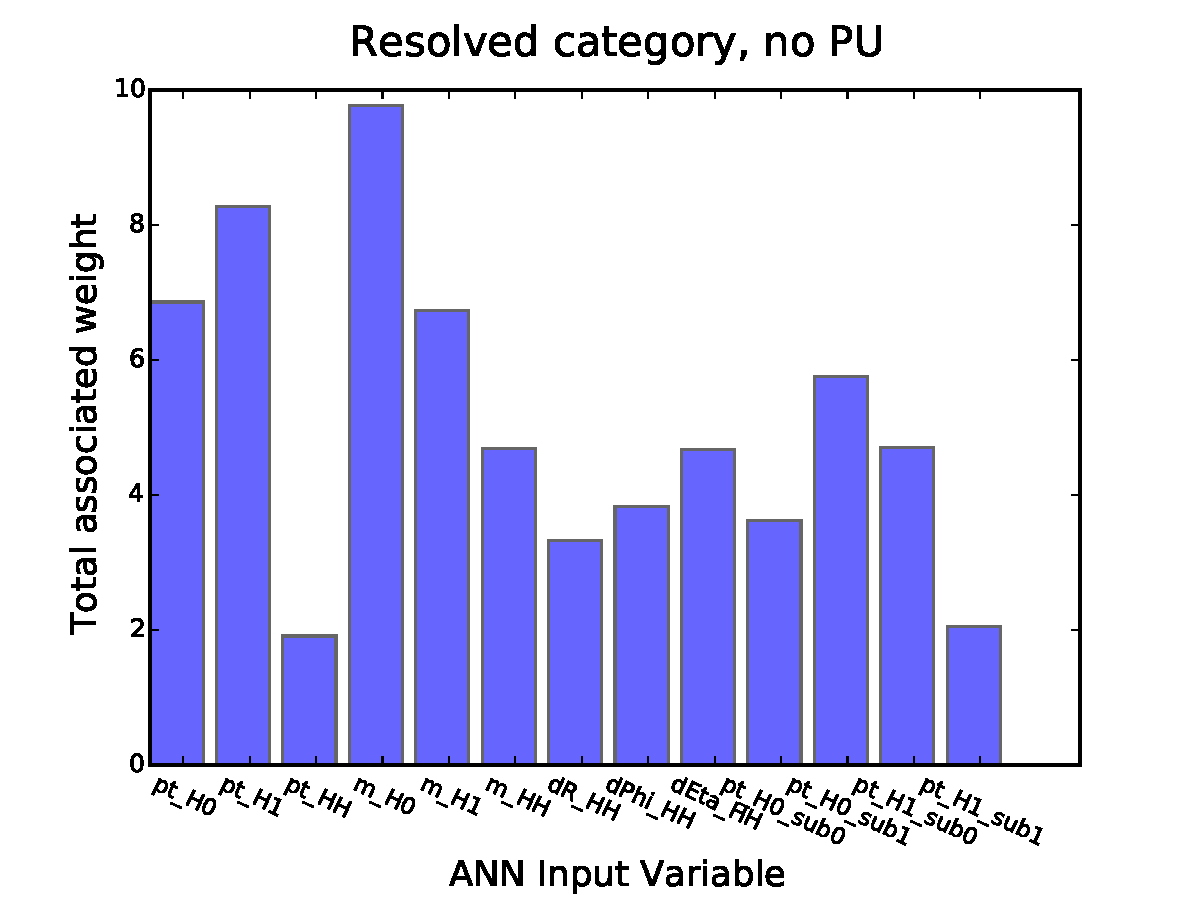
\includegraphics[width=0.49\textwidth]{plots/res_wgthist_noPU.pdf}
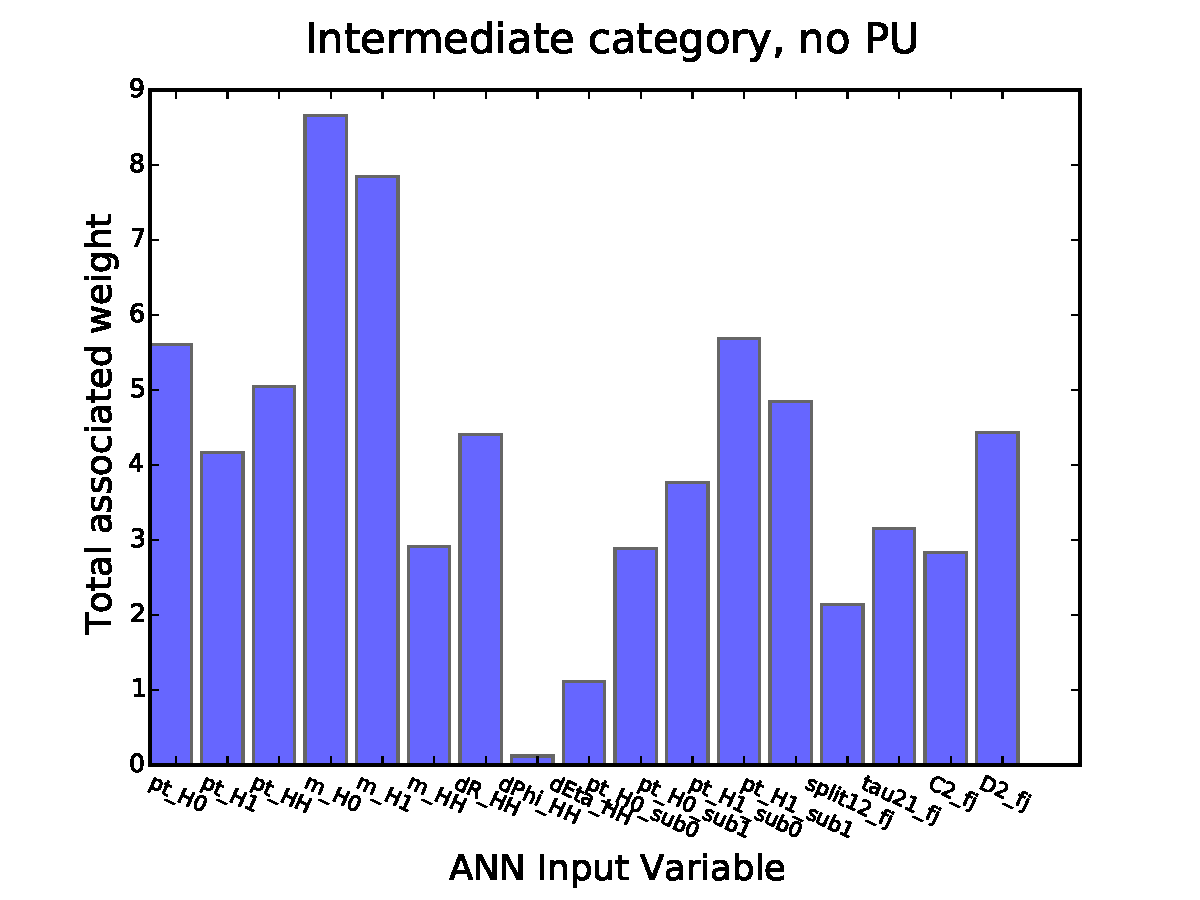
\includegraphics[width=0.49\textwidth]{plots/int_wgthist_noPU.pdf}
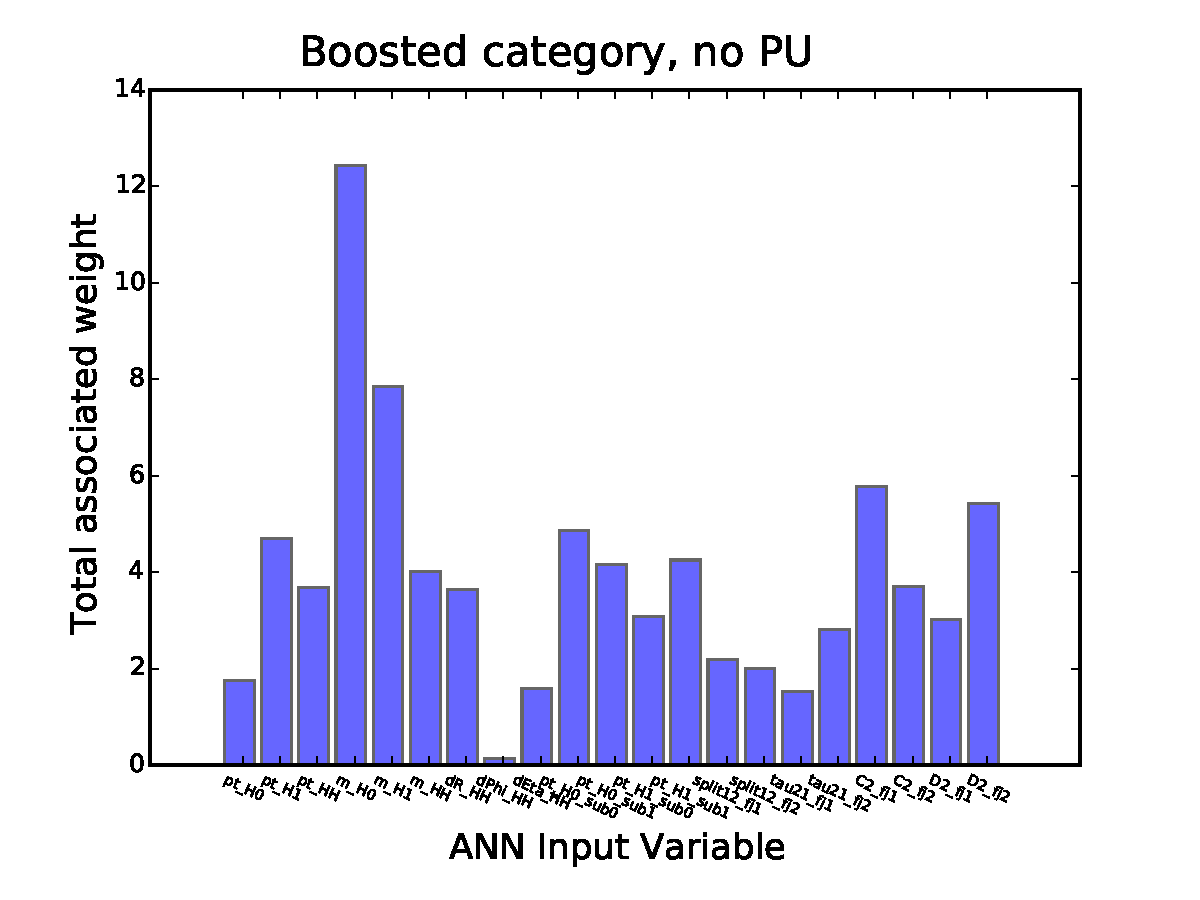
\includegraphics[width=0.60\textwidth]{plots/bst_wgthist_noPU.pdf}
\vspace{-0.5cm}
\caption{\small
Distribution of the total associated weight,
Eq.~(\ref{eq:totweight}) for each of the $N_{\rm var}$ input
variables of the resolved (upper left),  intermediate (upper right)
and boosted (lower plot)
categories.
}
\label{fig:nnweights}
\end{center}
\end{figure}
%%%%%%%%%%%%%%%%%%%%%%%

%
In Fig.~\ref{fig:nnweights} we show
the distribution of the total associated weight,
Eq.~(\ref{eq:totweight}) for each of the $N_{\rm var}$ input
variables of the three categories, using the
notation for the kinematic variables
as in Sect.~\ref{sec:input}.
%
In the 
resolved category, the variables that carry 
a higher discrimination power
are the transverse momentum of the two reconstructed Higgs candidates and
their invariant masses.
%
In the case of the boosted category, the invariant mass distribution
of the Higgs candidates is also the most discriminatory
variable, followed by the subjet $p_T$ distributions and
substructure variables such as $C_2^{(\beta)}$ and
$D_2^{(\beta)}$.

%%%%%%%%%%%%%%%%%%%%%%%%
\begin{figure}[t]
\begin{center}
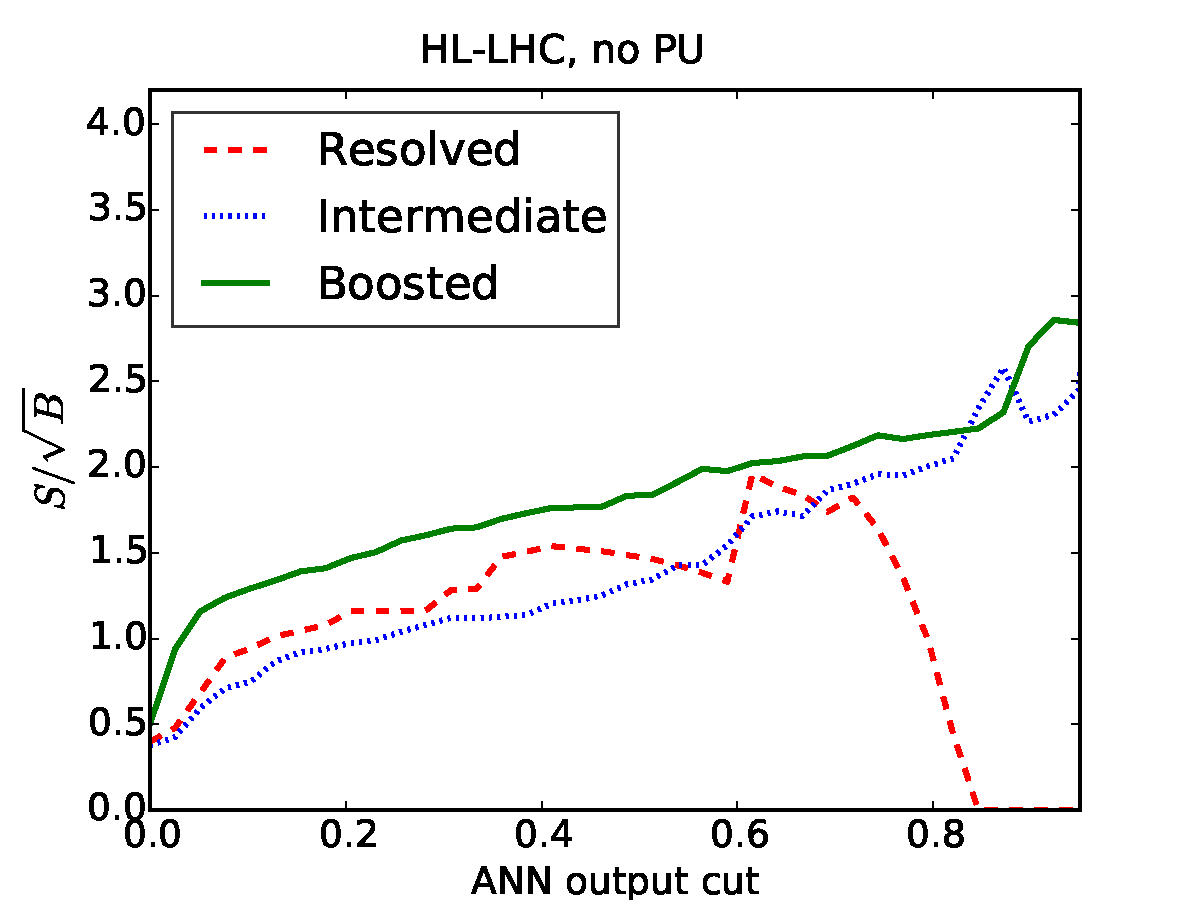
\includegraphics[width=0.48\textwidth]{plots/ssb_noPU.pdf}
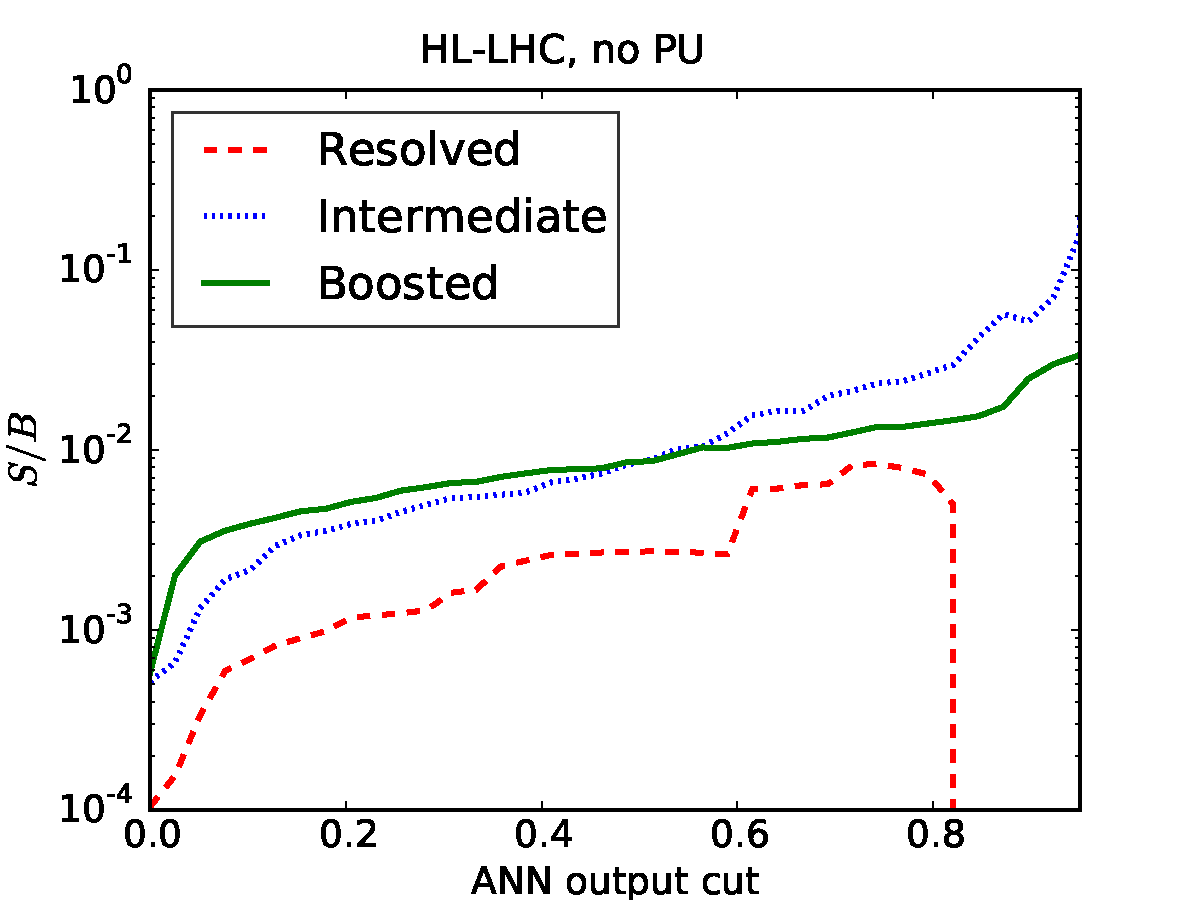
\includegraphics[width=0.48\textwidth]{plots/sb_noPU.pdf}
\caption{\small
  The values of the signal significance, $S/\sqrt{B}$, and of the
  signal over background ratio, $S/B$, for the boosted, intermediate
  and resolved categories as a function of the cut
  $y_{\rm cut}$ in the ANN output.
  %
  The $y_{\rm cut}=0$
  results are those at the end of the cut-based
  analysis.
}
\label{fig:sb_mva}
\end{center}
\end{figure}
%%%%%%%%%%%%%%%%%%%%%%%

The results for the signal significance $S/\sqrt{B}$ and
the signal over background ratio
$S/B$ as a function of $y_{\rm cut}$
for the three categories are given in 
Fig.~\ref{fig:sb_mva}.
%
The values 
for $y_{\rm cut}=0$ correspond to those at
the end of the loose cut-based analysis.
%
We observe how in the three
 categories there is a marked  improvement in signal
significance as compared to the pre-MVA results.
%
We also observe a substantial enhancement in $S/B$, arising
from the background suppression achieved by the MVA, reaching
values of 1\%, 6\% and 3.5\% in the resolved,
intermediate and boosted categories.
%
This improvement in $S/B$ is crucial to ensure the feasibility
of this measurement, since it allows systematic
uncertainties in the background determination to
be at most of a similar size.

%
The optimal value of the cut in the
ANN output, $y_{\rm cut}$,  can be determined from the maximisation of $S/\sqrt{B}$,
ensuring that the number of signal events $N_{\rm ev}$
expected at the HL-LHC does not become too low.
%
In  addition, we require
that the number of MC events used to define the signal
category (events with $y_i \ge y_{\rm cut}$)
is sufficiently large in order to avoid the biases and statistical
fluctuations associated to a small training sample.
%
In Table~\ref{table:cutflowMVA} we quote, for the optimal
value of $y_{\rm cut}$
in each category,
the number of signal and background events $N_{\rm ev}$ expected
at the HL-LHC, as well as $S/\sqrt{B}$ and $S/B$.
%
For completeness, we also include the corresponding
pre-MVA results.
%

%%%%%%%%%%%%%%%%%%%%%%%%%%%%%%%%%%%%%%%%%%%%%%%%%%%%%%%%%%%%%%%%%%%%%%%%%%%%
\begin{table}[t]
  \centering
  \begin{tabular}{|c|l|c|c|c|c|}
    \hline
    \multicolumn{6}{|c|}{HL-LHC, no PU} \\
    \hline
    \hline
    Category  &   &  $N_{\rm ev}$ signal &  $N_{\rm ev}$ back  &  $S/\sqrt{B}$ & $S/B$ \\ 
    \hline
    \hline
    \multirow{2}{*}{Boosted} &  $y_{\rm cut}=0$  & 440 & $7.6\cdot 10^5$  & 0.5  & $6\cdot 10^{-4}$  \\
    &  $y_{\rm cut}=0.90$ & 290  & $1.2\cdot 10^4$   & 2.7  & 0.03 \\
    \hline
    \hline
    \multirow{2}{*}{Intermediate} &  $y_{\rm cut}=0$  & 280   & $5.3\cdot 10^5$
    & 0.4 & $5\cdot 10^{-4}$ \\
    &  $y_{\rm cut}=0.85$ & 130  & $3.1\cdot 10^3$  & 2.3 & 0.04\\
    \hline
    \hline
      \multirow{2}{*}{Resolved} &  $y_{\rm cut}=0$  & 1500 &  $1.5\cdot 10^{7}$ &  0.4 &$1\cdot 10^{-4}$ \\
    &  $y_{\rm cut}=0.60$ & 630  & $1.1\cdot 10^{5}$ & 1.9 & 0.01 \\
    \hline
      \end{tabular}
  \caption{\small Post-MVA results, for the optimal value of the
    ANN discriminant $y_{\rm cut}$ in the three categories, compared with the
    corresponding
    pre-MVA results ($y_{\rm cut}=0$).
    %
    We quote the number of signal and
    background events expected for $\mathcal{L}=3$ ab$^{-1}$,
    the signal significance $S/\sqrt{B}$ and
    the signal over background ratio $S/B$.
    %
    The pre-MVA results correspond to row C2 in
    Table~\ref{tab:cutflow_noPU_1}.
    \label{table:cutflowMVA}
  }
\end{table}
%%%%%%%%%%%%%%%%%%%%%%%%%%%%%%%%%%%%%%%%%%%%%%%%%%%%%%%%%%%%%%%%%%%%%%%%%%%%

From Table~\ref{table:cutflowMVA} we see that
following the application of the MVA, 
the signal significance in the boosted category increases
from 0.5 to 2.7, with $S/B$ increasing from $0.06\%$ to $3\%$.
%
For the intermediate and resolved categories, $S/\sqrt{B}$
increases from 0.4 to 2.3 and 1.9 respectively, with
the signal over background ratio raising from
$0.05\%$ and $0.01\%$ to 4\% and 1\%.
%
Combining the three categories, taking into
account all background components, we obtain the overall signal
significance:
\be
\lp \frac{S}{\sqrt{B}}\rp_{\rm tot} \simeq 4.0~(1.3) \, ,\quad
\mathcal{L}=3000~(300)\,{\rm fb}^{-1}\, ,
\ee
%
The signal significance for
$\mathcal{L}=3$ ab$^{-1}$
is thus
well above the threshold for the observation of Higgs
pair production.
%
However, given that the HL-LHC will be a high-PU environment,
which will affect the description of the various
kinematic distributions used as input to the MVA,
it is essential to quantify the robustness of these
results
in a realistic environment including the effects of
significant PU.


%%%%%%%%%%%%%%%%%%%%%%%%%%%%%%%%%%%%%

It should be emphasized that MVAs such as the ANNs used in this work can always be understood as
a combined set of correlated cuts.
%
Once the ANNs have been trained, it is possible to compare  kinematical distributions after and before the ANN  cut to verify its impact.
%
This information would allow in principle to perform a cut-based analysis, without the need of using ANNs,
and finding similar results.


To illustrate this point,
in Fig.~\ref{fig:pt_H0_sub0_res_noPU_ANNcut} we show
the $p_T$ distribution of the leading AKT04 small-$R$ jets
and the invariant mass of reconstructed Higgs candidates in the resolved
  category, comparing the pre-MVA results ($y_{\rm cut}=0$) with the post-MVA
  results ($y_{\rm cut}=0.60$) for signal and background  events.
  %
  The distributions are not normalized, to better visualize the effect
  of the MVA cut.
  %
  Unsurprisingly, the ANN cut effectively selects events which
  lead to similar kinematical distributions between signal
  and background events.
  %
  In the case of the small-$R$ jets $p_T$ distribution, the
  ANN cuts favors the
  high-$p_T$ region, while for the invariant mass distribution
  only the region around the Higgs mass peak is selected for
  background events.


%%%%%%%%%%%%%%%%%%%%%%%%
\begin{figure}[t]
\begin{center}
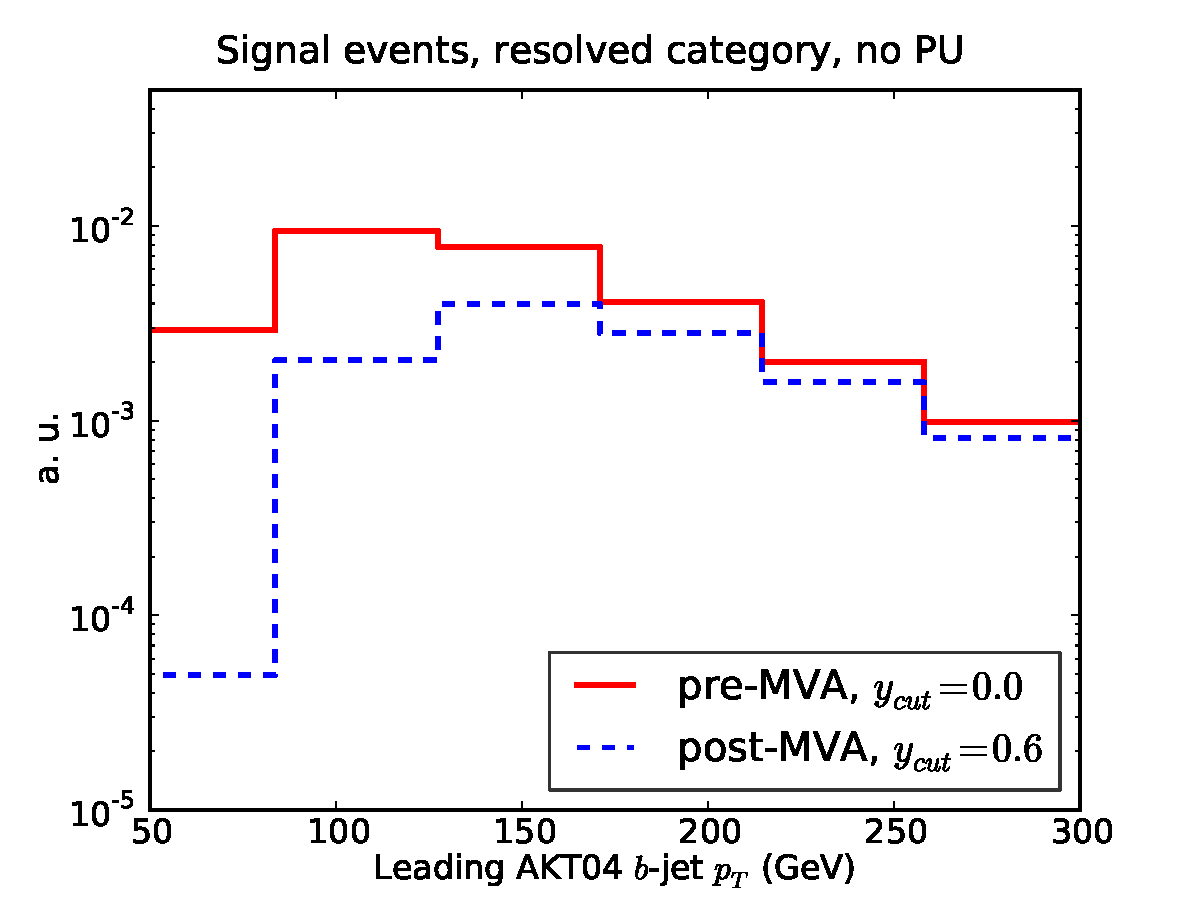
\includegraphics[width=0.48\textwidth]{plots/pt_H0_sub0_res_noPU_ANNcut.pdf}
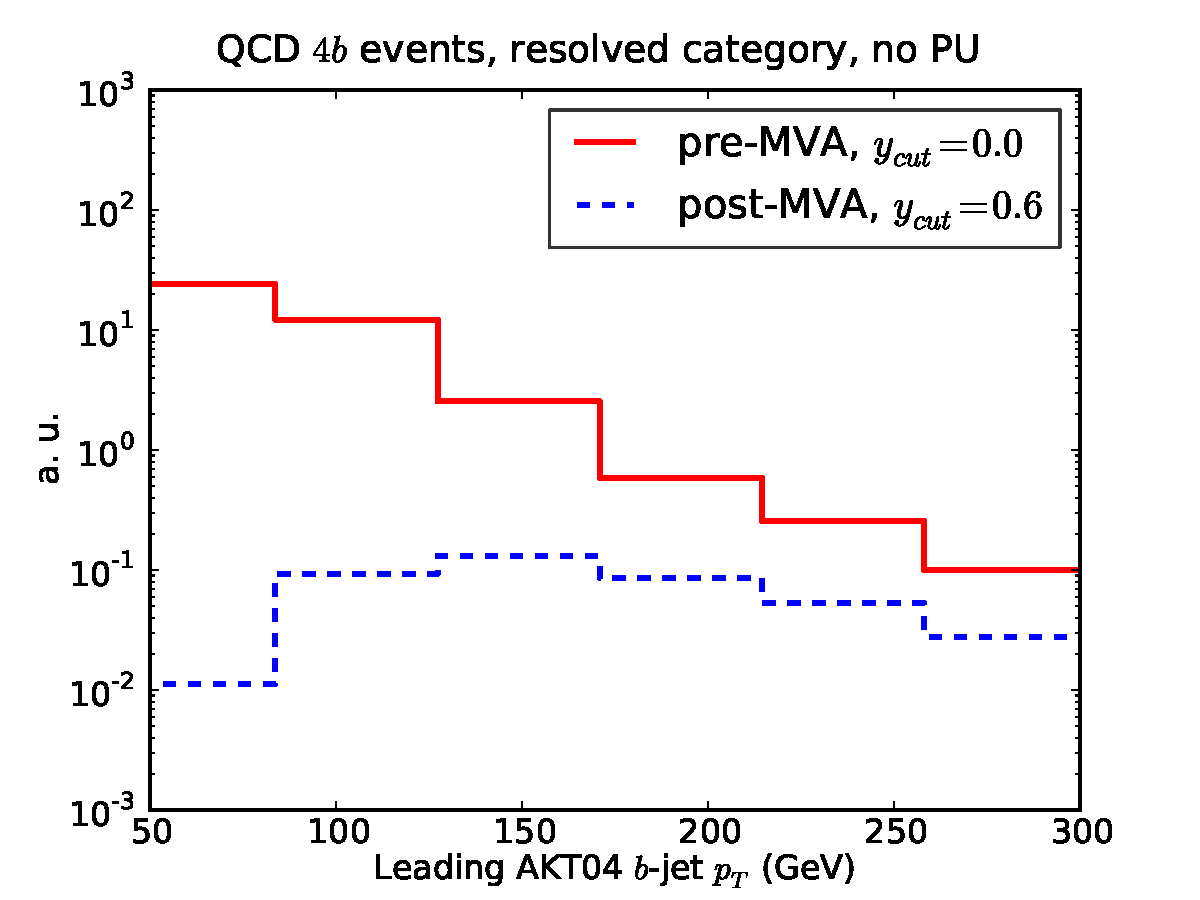
\includegraphics[width=0.48\textwidth]{plots/pt_H0_sub0_res_noPU_ANNcut_back_4b.pdf}
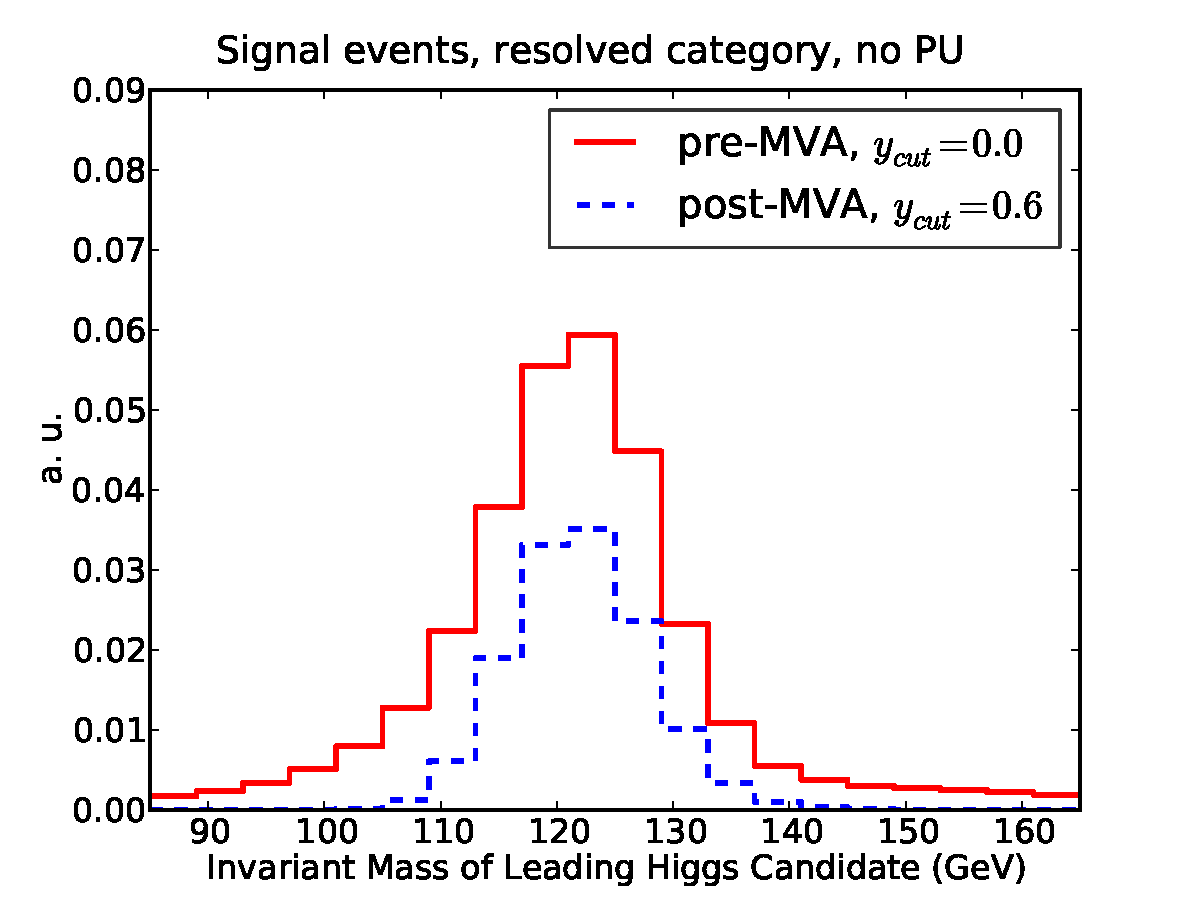
\includegraphics[width=0.48\textwidth]{plots/m_H0_res_noPU_ANNcut.pdf}
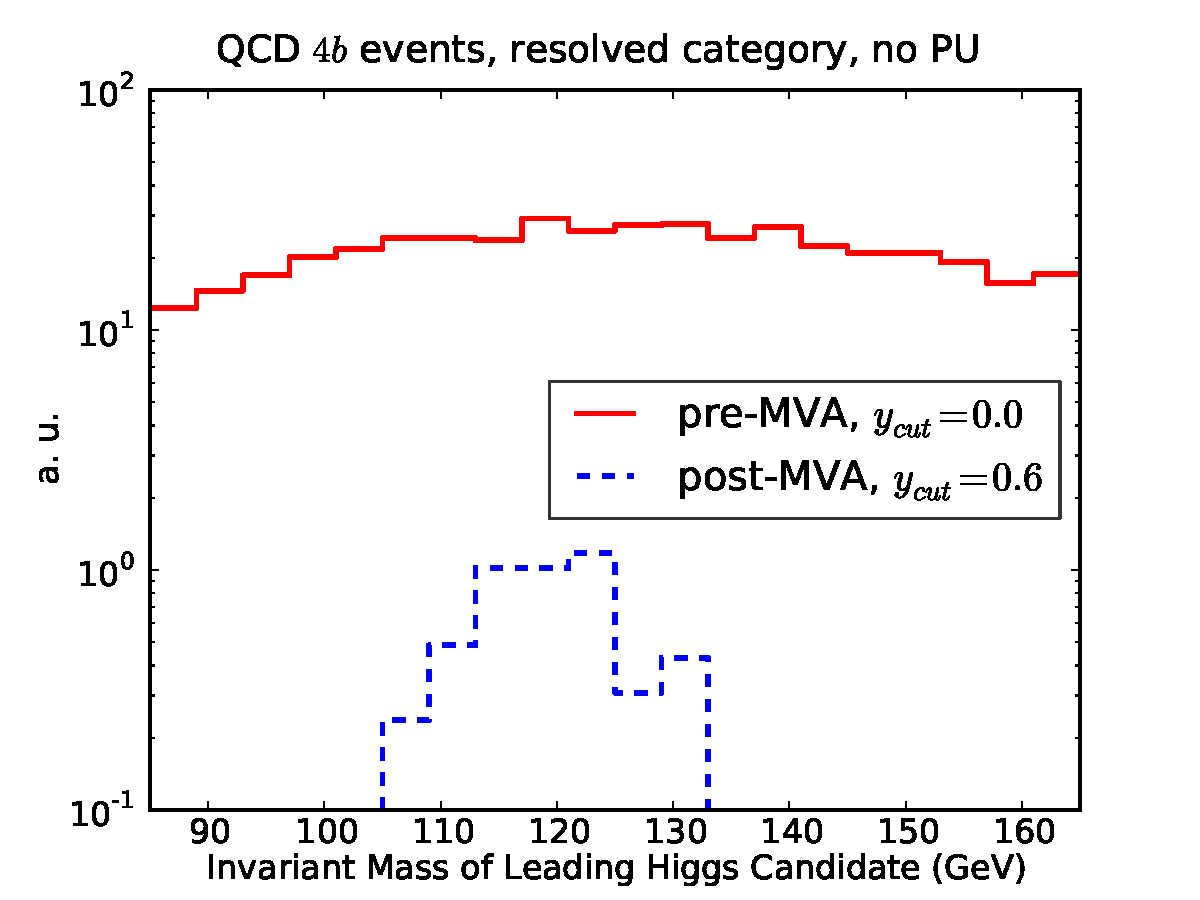
\includegraphics[width=0.48\textwidth]{plots/m_H0_res_noPU_ANNcut_back_4b.pdf}
\caption{\small
  The $p_T$ distribution of the leading AKT04 small-$R$ jets (upper plots)
  and
  the invariant mass of reconstructed Higgs candidates (lower plots) in the resolved
  category, comparing the pre-MVA results ($y_{\rm cut}=0$) with the post-MVA
  results ($y_{\rm cut}=0.60$) for signal (left) and background (right plot) events.
  %
  In this case the distributions are not normalized, to better visualize the effects
  of the MVA cut.
}
\label{fig:pt_H0_sub0_res_noPU_ANNcut}
\end{center}
\end{figure}
%%%%%%%%%%%%%%%%%%%%%%%



\subsection{Impact of PU in the MVA}

In this section we study how the MVA results are modified
when the analysis is performed including significant PU.
%
The loose cut-based analysis and the subsequent
MVA optimization have been performed using the same
settings as in the case without PU.
%
In Table~\ref{tab:cutflow_PU80_1}
we provide the pre-MVA cut flow in the case of PU80,
the corresponding version without PU being
Table~\ref{tab:cutflow_noPU_1}.
%
The interplay between the signal cross-sections and the various
background components is qualitatively unchanged as compared
to the no PU case.

%%%%%%%%%%%%%%%%%%%%%%%%%%%%%%%%%%%%%%%%%%%%%%%%%
\begin{table}[t]
  \centering
  \scriptsize
      \begin{tabular}{|l|cc|cccc|cccc|}
  \hline
\multicolumn{11}{|c|}{Resolved category, $\la n_{\rm PU}\ra=80$+SK}\\
\hline
&  \multicolumn{6}{c|}{Cross-section [fb]} &  &  & &  \\
   &  $hh\to 4b$ &  total bkg  &   $4b$    &  $2b2j$   &   $4j$    &
$t\bar{t}$ &
$S/B_{\rm tot}$ & $S/B_{\rm 4b}$ & $S/\sqrt{B_{\rm tot}}$ & $S/\sqrt{B_{\rm 4b}}$ \\
  \hline
  \hline
  C0    &    $39 $ &   $5.2 \cdot 10^9$   & $1.8 \cdot 10^6$ & $3.5 \cdot 10^8$ & $4.9 \cdot 10^9$ & $3.5 \cdot 10^5$     &  $ 7.5 \cdot 10^{-9}$   & $2.2 \cdot 10^{-5}$  &
  $3.0 \cdot 10^{-2}$   & $1.6 $  \\
 C1a   &    $39$&   $5.2 \cdot 10^9$   & $1.8 \cdot 10^6$ & $3.5 \cdot 10^8$ & $4.9 \cdot 10^9$ & $3.5 \cdot 10^5$     &  $7.5 \cdot 10^{-9}$   & $2.2 \cdot 10^{-5}$   &   $3.0 \cdot 10^{-2}$   & $1.6  $ \\
 C1b   &  $26$ &   $4.4 \cdot 10^8$   & $1.5 \cdot 10^5$ & $3.0 \cdot 10^7$ & $4.1 \cdot 10^8$ & $2.6 \cdot 10^5$     &  $ 5.9 \cdot 10^{-8}$   & $1.7 \cdot 10^{-4}$  &    $6.7 \cdot 10^{-2}$   & $3.6  $\\
 C1c   &   $26$  &   $4.4 \cdot 10^8 $  & $1.5 \cdot 10^5$ & $3.0 \cdot 10^7$ & $4.1 \cdot 10^8$ & $2.6 \cdot 10^5$     &    $5.9 \cdot 10^{-8}$   & $1.7 \cdot 10^{-4}$  &     $ 6.7 \cdot 10^{-2}$   &$ 3.6 $ \\
 C1d   &   $7.4$ &   $1.1 \cdot 10^8$   & $4.2 \cdot 10^4$ & $7.7 \cdot 10^6$ & $9.9 \cdot 10^7$ & $1.1 \cdot 10^5$     &   $6.9 \cdot 10^{-8}$   & $1.8 \cdot 10^{-4}$   &   $3.9 \cdot 10^{-2}$   & $2.0 $ \\
 C2    &  $1.4$ &   $9.0 \cdot 10^3$   & $3.5 \cdot 10^3$ & $5.1 \cdot 10^3$ & $3.1 \cdot 10^2$ & $5.0 \cdot 10^1$     &    $1.6 \cdot 10^{-4}$   & $4.1 \cdot 10^{-4}$  &   $0.84$   &
 $1.3 $ \\
\hline
\end{tabular}
  $\,$ \\
  \vspace{0.5cm}
 \begin{tabular}{|l|cc|cccc|cccc|}
  \hline
\multicolumn{11}{|c|}{Intermediate category, $\la n_{\rm PU}\ra=80$+SK+Trim}\\
\hline
&  \multicolumn{6}{c|}{Cross-section [fb]} &  &  & &  \\
   &  $hh\to 4b$ &  total bkg  &   $4b$    &  $2b2j$   &   $4j$    &
$t\bar{t}$ &
$S/B_{\rm tot}$ & $S/B_{\rm 4b}$ & $S/\sqrt{B_{\rm tot}}$ & $S/\sqrt{B_{\rm 4b}}$ \\
  \hline
  \hline
 C0      &  $39$  &   $5.2 \cdot 10^9$   & $1.8 \cdot 10^6$ & $3.5 \cdot 10^8$ & $4.9 \cdot 10^9$ & $3.5 \cdot 10^5$     &    $7.5 \cdot 10^{-9}$   & $2.2 \cdot 10^{-5}$  &   $3.0 \cdot 10^{-2}$   & $1.6 $ \\
 C1b     &  $6.7$  &   $8.1 \cdot 10^7$   & $2.1 \cdot 10^4$ & $5.2 \cdot 10^6$ & $7.6 \cdot 10^7$ & $3.0 \cdot 10^4$     &   $8.3 \cdot 10^{-8}$   & $3.2 \cdot 10^{-4}$   &   $4.1 \cdot 10^{-2}$   & $2.5 $ \\
 C1c     & $6.4 $  &   $6.2 \cdot 10^7 $  & $1.5 \cdot 10^4$ & $3.9 \cdot 10^6$ & $5.8 \cdot 10^7$ & $2.8 \cdot 10^4$     &    $1.0 \cdot 10^{-7}$   & $4.2 \cdot 10^{-4}$  &   $4.5 \cdot 10^{-2}$   & $2.8 $ \\
 C1d     & $1.2 $  &   $2.8 \cdot 10^6$   & $7.9 \cdot 10^2$ & $1.9 \cdot 10^5$ & $2.7 \cdot 10^6$ & $6.5 \cdot 10^3$     &     $4.3 \cdot 10^{-7}$   & $1.5 \cdot 10^{-3}$  &   $3.9 \cdot 10^{-2}$   & $2.4 $ \\
 C2      & $0.21$  &   $2.6 \cdot 10^2$   & $47$ & $1.8 \cdot 10^2$ & $30$ & $2.2 $     &   $  8.2 \cdot 10^{-4}$   & $4.5 \cdot 10^{-3}$  &   $0.72$   & $1.7 $ \\
\hline
\end{tabular}
  $\,$ \\
 \vspace{0.5cm}
 \begin{tabular}{|l|cc|cccc|cccc|}
  \hline
\multicolumn{11}{|c|}{Boosted category, $\la n_{\rm PU}\ra=80$+SK+Trim}\\
\hline
&  \multicolumn{6}{c|}{Cross-section [fb]} &  &  & &  \\
   &  $hh\to 4b$ &  total bkg  &   $4b$    &  $2b2j$   &   $4j$    &
$t\bar{t}$ &
$S/B_{\rm tot}$ & $S/B_{\rm 4b}$ & $S/\sqrt{B_{\rm tot}}$ & $S/\sqrt{B_{\rm 4b}}$ \\
  \hline
  \hline
C0      &  $39$  &   $5.2 \cdot 10^9$   & $1.8 \cdot 10^6$ & $3.5 \cdot 10^8$ & $4.9 \cdot 10^9$ &  $3.5 \cdot 10^5$     &    $7.5 \cdot 10^{-9}$   & $2.2 \cdot 10^{-5}$  &   $3.0 \cdot 10^{-2}$   & $1.6 $ \\
 C1a     & $39$  &   $5.2 \cdot 10^9 $  & $1.8 \cdot 10^6$ & $3.5 \cdot 10^8$ & $4.9 \cdot 10^9$ & $3.5 \cdot 10^5  $   &    $7.5 \cdot 10^{-9}$   & $2.2 \cdot 10^{-5}$ &   $3.0 \cdot 10^{-2}$   & $1.6 $  \\
 C1b     &  $8.5 $  &   $4.1 \cdot 10^7$   & $1.0 \cdot 10^4$ & $2.7 \cdot 10^6$ & $3.8 \cdot 10^7$ & $2.0 \cdot 10^4 $    &   $2.1 \cdot 10^{-7}$   & $8.2 \cdot 10^{-4}$  &  $7.3 \cdot 10^{-2}$   & $4.6 $ \\
 C1c     & $6.0 $  &   $3.2 \cdot 10^7$   & $6.8 \cdot 10^3$ & $1.9 \cdot 10^6$ & $3.0 \cdot 10^7$ & $1.9 \cdot 10^4  $   &   $1.9 \cdot 10^{-7}$   & $8.8 \cdot 10^{-4}$ &    $5.8 \cdot 10^{-2}$   & $4.0 $ \\
 C1d     & $2.0 $ &   $2.2 \cdot 10^6$   & $5.4 \cdot 10^2$ & $1.4 \cdot 10^5$ & $2.0 \cdot 10^6$ & $4.8 \cdot 10^3   $  &   $9.4 \cdot 10^{-7}$   & $3.8 \cdot 10^{-3}$ & $7.6 \cdot 10^{-2}$   & $4.8 $ \\
 C2      & $0.34$  &   $1.5 \cdot 10^2$   & $40$ & $86$ & $22$ & $1.8 $     &   $ 2.2 \cdot 10^{-3}$   & $8.5 \cdot 10^{-3}$ &   $1.5 $   & $2.9 $ \\
\hline
\end{tabular}
%%%%%%%%%%%%%%%%%%%%%%%%%%%%%%%%%%%%%%%%%%%%%%%%%%%%%%%%%%%%%%%
 

    \caption{\small Same as Table~\ref{tab:cutflow_noPU_1},
now for the case
    of PU80+SK+Trim.
 \label{tab:cutflow_PU80_1}}
\end{table}
%%%%%%%%%%%%%%%%%%%%%%%%%%%%%%%%%%%%

In Table~\ref{table:cutflowMVA_PU} we compare the results
for the PU80+SK+Trim case between
  the pre-MVA loose cut-based analysis and
  the post-MVA results for the
  optimal values of the ANN output cut $y_{\rm cut}$.
  %
  As in Table~\ref{table:cutflowMVA}, 
  we also quote 
   the number of signal and
    total background events expected
   for $\mathcal{L}=3$ ab$^{-1}$
    and the values of $S/\sqrt{B}$ and $S/B$.
%
We observe that the pre-MVA 
signal significance is close
to the results of the simulations
without PU for the three categories.
%
We now find values for $S/\sqrt{B}$ of 0.4, 0.3 and 0.6, in the resolved,
intermediate and boosted categories, respectively, to be compared
with the corresponding values without PU, namely 0.4, 0.4 and 0.5.
%
The number of selected
signal events in each category at the
end of the cut-based analysis is only mildly affected
by PU.
%
The slight pre-MVA improvement in $S/\sqrt{B}$ for the
boosted case arises from a reduction in the number
of background events that are classified in this category
as compared to the case without PU.

Once the MVA is applied, the signal significance in the 
resolved, intermediate and boosted
categories increases to 2.0, 1.9 and 1.5 respectively,
to be compared with the corresponding values
without PU, namely 1.9, 2.3 and 2.7.
%
Therefore, the post-MVA effect of PU on $S/\sqrt{B}$ is
a moderate degradation of the boosted and intermediate categories,
specially for the former,
while the resolved category is largely unchanged.\footnote{
  The impact of PU on the  separate significance of
  the three categories exhibits some
  dependence on the specific choice for $n_{\rm PU}$  and on the settings
  of the PU subtraction strategy.
  %
  We find however that the
  overall signal significance from combining the three
  categories is similar in the $n_{\rm PU}=80$ and
  $n_{\rm PU}=150$ cases.
}
%
We also observe that, due
to the MVA, the
signal over background ratio is increased from 0.007\%, 0.03\% and
0.1\% up to 1\%, 3\% and 1\% in the resolved, intermediate
and boosted categories respectively.
%
This indicates that while this measurement is still highly challenging,
requiring a careful extraction of the QCD
background from the data, it should be within reach.

%%%%%%%%%%%%%%%%%%%%%%%%%%%%%%%%%%%%%%%%%%%%%%%%%%%%%%%%%%%%%%%%%%%%%%%%%%%%
\begin{table}[t]
  \centering
  \begin{tabular}{|c|l|c|c|c|c|}
        \hline
     \multicolumn{6}{|c|}{HL-LHC, PU80+SK+Trim} \\
     \hline
         \hline
    Category  &   &  $N_{\rm ev}$ signal &  $N_{\rm ev}$ back  &  $S/\sqrt{B}$ & $S/B$ \\ 
    \hline
    \hline
    \multirow{2}{*}{Boosted} &  $y_{\rm cut}=0$  & 410   &  $4.5\cdot 10^5$ & 0.6   & $ 10^{-3}$  \\
    &  $y_{\rm cut}=0.8$ &  290  & $3.7\cdot 10^4$  & 1.5    & 0.01  \\
    \hline
    \hline
    \multirow{2}{*}{Intermediate} &  $y_{\rm cut}=0$  &  260  & $7.7\cdot 10^5$    & 0.3    &
     $3\cdot 10^{-4}$ \\
    &  $y_{\rm cut}=0.75$ & 140 & $5.6\cdot 10^3$  &  1.9   & 0.03 \\
    \hline
    \hline
    \multirow{2}{*}{Resolved} &  $y_{\rm cut}=0$  &  1800  & $2.7\cdot 10^7$
    & 0.4    &  $7\cdot 10^{-5}$  \\
    &  $y_{\rm cut}=0.60$ & 640  & $1.0\cdot 10^5$  &  2.0   & 0.01  \\
    \hline
      \end{tabular}
  \caption{\small Same as Table~\ref{table:cutflowMVA}, now for the case
    of PU80+SK+Trim.
        \label{table:cutflowMVA_PU}
  }
\end{table}
%%%%%%%%%%%%%%%%%%%%%%%%%%%%%%%%%%%%%%%%%%%%%%%%%%%%%%%%%%%%%%%%%%%%%%%%%%%%

%%%%%%%%%%%%%%%%%%%%%%%%%%%%%%%%%%%%%%%%%%%%%
\begin{figure}[t]
  \begin{center}
    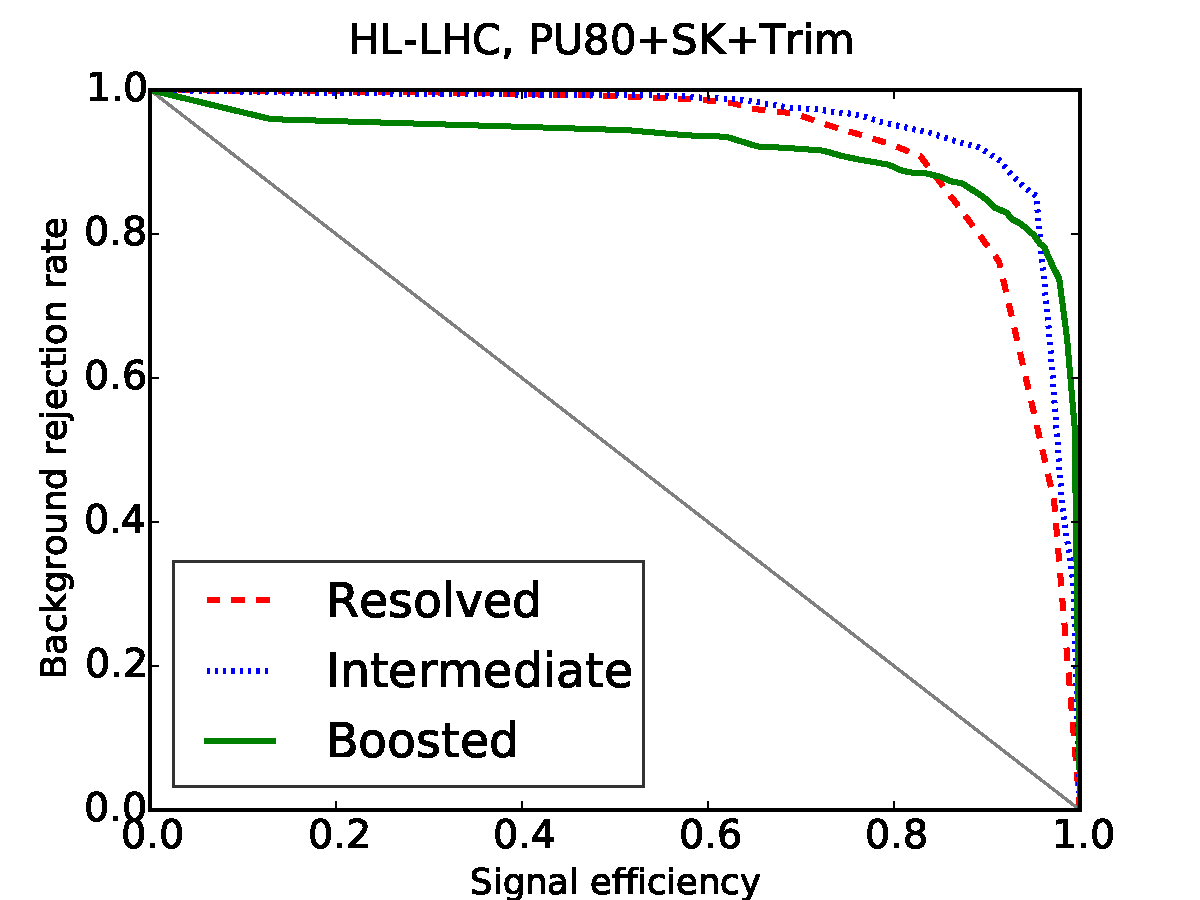
\includegraphics[width=0.49\textwidth]{plots/roc_SKPU80.pdf}
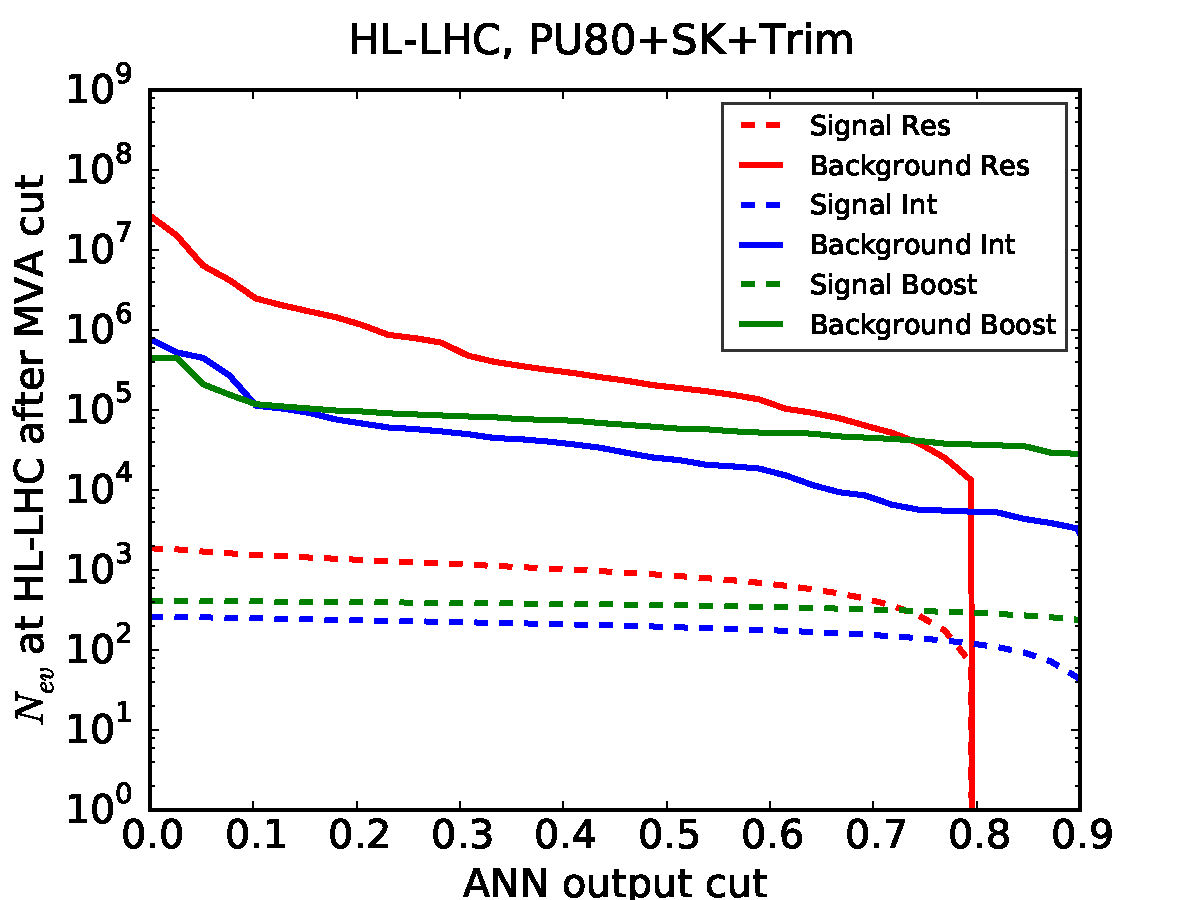
\includegraphics[width=0.49\textwidth]{plots/nev2_SKPU80.pdf}
\caption{\small Same as Fig.~\ref{fig:nev2}
 for
 the PU80+SK+Trim case.
\label{fig:nev2_PU}}
\end{center}
\end{figure}
%%%%%%%%%%%%%%%%%%%%%%%%%%%%%%%%%%%%%

In Fig.~\ref{fig:nev2_PU}
we show the number of signal and background events that
are expected for $\mathcal{L}=3$ ab$^{-1}$
as a function of
$y_{\rm cut}$, together with the corresponding ROC curve.
%
The slight degradation of the boosted category in the case
of PU can be seen by comparing with the corresponding
results without PU in Fig.~\ref{fig:nev2}.
%
In Fig.~\ref{fig:sb_mva_PU} we show the signal significance,
$S/\sqrt{B}$, and the signal over background ratio,
$S/B$, accounting now for the effects of PU.
%
The corresponding results in the case without PU were shown in
Fig.~\ref{fig:sb_mva}.
%
As can be seen, the MVA-driven enhancement remains robust in the
presence of PU, with $S/\sqrt{B}$ only moderately degraded.
%
Therefore, the qualitative conclusions drawn
in the case without PU also hold when the analysis
is performed in a high-PU environment.
%
Since no specific effort has been performed to
optimize PU subtraction, for instance by tuning the values
of the patch length $a$ in {\tt SoftKiller}
or the $p_T$ threshold during jet trimming,
we believe that
there should be still room for further improvement.

%%%%%%%%%%%%%%%%%%%%%%%%%%%%%%%%%%%%%%%%%%%%%%%%%%%%
\begin{figure}[t]
\begin{center}
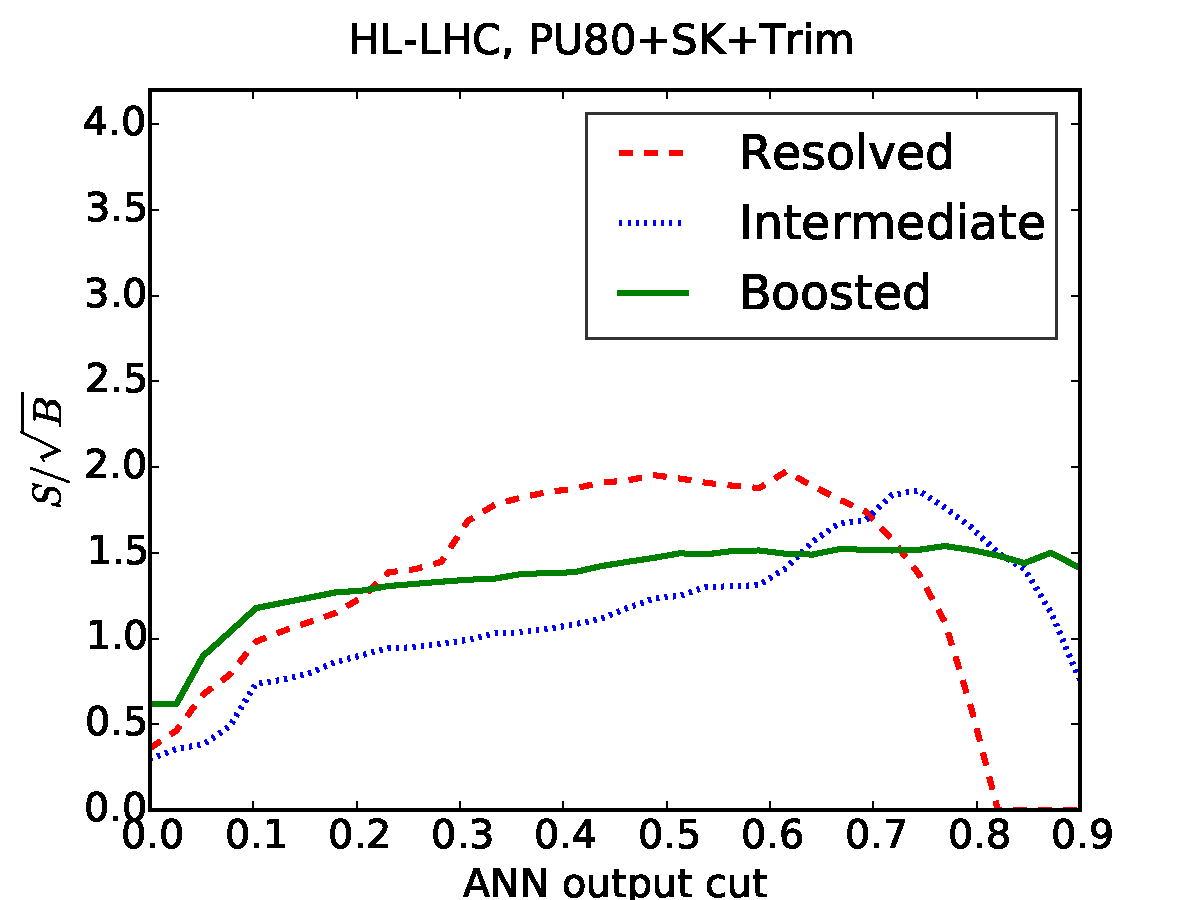
\includegraphics[width=0.48\textwidth]{plots/ssb_SKPU80.pdf}
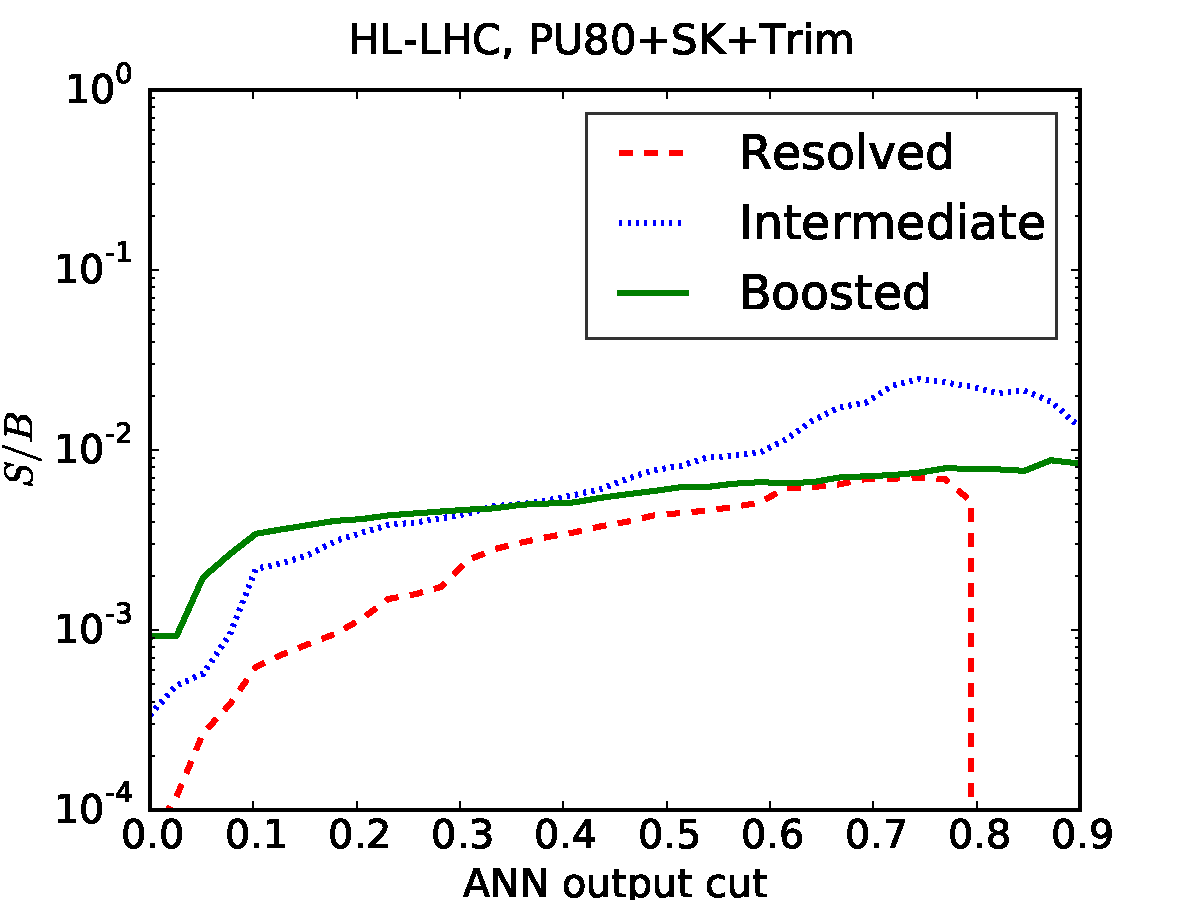
\includegraphics[width=0.48\textwidth]{plots/sb_SKPU80.pdf}
\caption{\small 
  Same as Fig.~\ref{fig:sb_mva} for
  the PU80+SK+Trim case.
}
\label{fig:sb_mva_PU}
\end{center}
\end{figure}
%%%%%%%%%%%%%%%%%%%%%%%

It is useful to quantify which of the MVA input variables
carry the highest discrimination power
in the case of PU, by means of
Eq.~(\ref{eq:totweight}),
and compare this with the corresponding
results without PU shown in Fig.~\ref{fig:nnweights}.
%
We have verified that 
the relative weight of the different input variables to the MVA
is mostly unchanged in the case of PU.
%
In the resolved category, the highest total associated weight is carried
by the Higgs candidates $p_T$ and invariant mass, as well
as by the $p_T$ of the individual small-$R$ jets.
%
For the boosted category, the highest weight is carried by the
Higgs invariant mass, followed by
the Higgs $p_T$, $m_{hh}$, the $p_T$ of the AKT03 subjets and the
substructure variables, with a similar weighting among them.

In Table~\ref{table:cutflowMVA_fakes} we provide
the post-MVA number of signal and background events  expected for
$\mathcal{L}=3$ ab$^{-1}$.
%
For the backgrounds, we quote
both
the total number, $N_{\rm ev}^{\rm tot}$,
and the  QCD $4b$ component only,
$N_{\rm ev}^{\rm 4b}$.
%
We quote results for the no PU and PU80+SK+Trim cases.
%
 We also quote in each case the corresponding values for the signal 
    significance and the signal over background ratio.
    %
    Note that the MVA is always trained to the inclusive background sample,
    though differences
    in the kinematic distributions of the $4b$ and $2b2j$ processes are
    moderate,
    see Fig.~\ref{fig:histoBack}.
    %
    From Table~\ref{table:cutflowMVA_fakes} one observes that
    all categories exhibit
    a marked improvement from eliminating the contamination
    from light and charm jet mis-identification.
    %
    For instance, in the intermediate category,
    $S/\sqrt{B}$ increases from 2.3 to 3.3 (1.9 to 2.9)
    in the no PU (PU80) case, with similar improvements in the
    resolved and boosted categories.
    %

%%%%%%%%%%%%%%%%%%%%%%%%%%%%%%%%%%%%%%%%%%%%%%%%%%%%%%%%%%%%%%%%%%%%%%%%%%%%
\begin{table}[t]
  \centering
  \scriptsize
  \begin{tabular}{|c|c|c|c|c||c|c||c|c|}
        \hline
        Category  &  &  signal  &  \multicolumn{2}{c||}{background}     &
        $S/\sqrt{B_{\rm tot}}$ & $S/\sqrt{B_{\rm 4b}}$  
        &  $S/B_{\rm tot}$ & $S/B_{\rm 4b}$\\
         &  &  $N_{\rm ev}$  &  $N_{\rm ev}^{\rm tot}$  &  $N_{\rm ev}^{\rm 4b}$   &
         &     &   &  \\
    \hline
    \hline
    \multirow{2}{*}{Boosted} &  no PU  & 290  & $1.2\cdot 10^4$  &  $8.0\cdot 10^3$    & 
      2.7 &  3.2  & 0.03 & 0.04 \\
      & PU80+SK+Trim & 290  &$3.7\cdot 10^4$ & $1.2\cdot 10^4$     &  1.5  & 2.7 &  0.01 & 0.02   \\
    \hline
    \hline
    \multirow{2}{*}{Intermediate} &  no PU   & 130   & $3.1\cdot 10^3$  & $1.5\cdot 10^3$    &
    2.3  & 3.3  &  0.04  & 0.08   \\
    & PU80+SK+Trim & 140 & $5.6\cdot 10^3$   & $2.4\cdot 10^3$   & 1.9  & 2.9  & 0.03 & 0.06  \\
    \hline
    \hline
    \multirow{2}{*}{Resolved} &   no PU  & 630 & $1.1\cdot 10^5$   & $5.8\cdot 10^4$
    & 1.9  & 2.7  & 0.01 & 0.01 \\
    & PU80+SK & 640  & $1.0\cdot 10^5$   & $7.0\cdot 10^4$   & 2.0 & 2.6  & 0.01 & 0.01 \\
    \hline
    \hline
    \multirow{2}{*}{\bf Combined} &   no PU  &  \multicolumn{3}{c||}{} 
    &  4.0 & 5.3  &   \multicolumn{2}{c|}{}  \\
    & PU80+SK+Trim &    \multicolumn{3}{c||}{}    & 3.1  & 4.7  &  \multicolumn{2}{c|}{}  \\
    \hline
      \end{tabular}
  \caption{\small Post-MVA number of signal and background events
    with  $\mathcal{L}=3$ ab$^{-1}$.
    %
    For the backgrounds, both the total number, $N_{\rm ev}^{\rm tot}$,
    and the  $4b$ 
    component only, $N_{\rm ev}^{\rm 4b}$, are shown.
     %
    Also provided are the values of the signal 
    significance and the signal over background ratio,
    both separated in categories and for their combination.
    %
    We quote the results without PU and for PU80+SK+Trim.
         \label{table:cutflowMVA_fakes}
  }
\end{table}
%%%%%%%%%%%%%%%%%%%%%%%%%%%%%%%%%%%%%%%%%%%%%%%%%%%%%%%%%%%%%%%%%%%%%%%%%%%%

In Table~\ref{table:cutflowMVA_fakes} we also provide
the results for $S/\sqrt{B}$ obtained by
combining the three categories.
%
Taking into
account all background components, we obtain for the case
of $n_{\rm PU}=80$
an overall signal
significance of
\be
\lp \frac{S}{\sqrt{B}}\rp_{\rm tot} \simeq 3.1~(1.0) \, ,\quad
\mathcal{L}=3000~(300)\,{\rm fb}^{-1}\, ,
\ee
%
indicating  that a measurement of
Higgs pair production in the $b\bar{b}b\bar{b}$ final state at the HL-LHC
should be 
above the threshold for observation, even when realistic PU conditions
are accounted for.
%
A similar signal significance is obtained in the case of
$n_{\rm PU}=150$.
%
Under the  assumption that
    the only relevant background would be the irreducible QCD $4b$ component,
    one obtains instead
    \be
\lp \frac{S}{\sqrt{B_{\rm 4b}}}\rp_{\rm tot} \simeq 4.7~(1.5) \, ,\quad
\mathcal{L}=3000~(300)\,{\rm fb}^{-1}\, .
\ee
%
Therefore, a measurement of Higgs pair production
in the $b\bar{b}b\bar{b}$ final state at the
HL-LHC  might be even above the threshold for discovery, provided
the effects due to mis-identification of light and charm jets as
$b$-jets can be reduced.
%
